\chapter{Pervasive Detection of Process Races in Deployed Systems}
\label{ch:racepro}

\section{Introduction} \label{racepro:sec:intro}

After presenting \scribe, our transparent record-replay engine most suited for
application debugging by capturing and reproducing hard to find bugs, we explore
ways to reveal dormant bugs in applications, and catch them before they happen.
Specifically, we explore the effect of bugs due to harmful process races in
software, and how to detect them using record-replay mechanisms.

While thread races have drawn much attention from the research
community~\cite{cui:tern:osdi10,racerx:sosp03,racefuzzer:pldi08,wu:loom:osdi10,yu:racetrack:sosp},
little has been done for \emph{process races}, where multiple
processes access an operating system (OS) resource such as a file or
device without proper synchronization.  
Process races are much broader than time-of-check-to-time-of-use
(\toctou) races or signal races~\cite{signal-race}.  A typical \toctou
race is an atomicity violation where the permission check and the use
of a resource are not atomic, so that a malicious process may slip in.
A signal race is often triggered when an attacker delivers two signals
consecutively to a process to interrupt and reenter a non-reentrant
signal handler.  In contrast, a process race may be any form of race.
Some real examples include a shutdown script that unmounts a file system
before another process writes its data, \code{ps | grep X} shows $N$
or $N+1$ lines depending on the timing of the two commands, and
\code{make -j} failures.

To better understand process races, we present the first study of real
process races.  We study hundreds of real applications across six
Linux distributions and show that process races are numerous and a real
threat to reliability and security.  For example, a simple search on
Ubuntu's software management site~\cite{launchpad} returns hundreds of 
process races.  Compared to thread races that typically corrupt volatile
application memory, process races are arguably more dangerous
because they often corrupt persistent and system resources.
Our study also reveals that some of their characteristics hint towards
potential detection methods.   

We then present \racepro, the first system for automatically detecting
process races beyond \toctou and signal races.  
\racepro faces three key challenges.  The first is scope:
process races are extremely heterogeneous.  They may involve many
different programs.  These programs may be written in different 
programming languages, run within different processes or threads,
and access diverse resources.  Existing detectors for thread or \toctou
races are unlikely to work well with this heterogeneity.

The second challenge is coverage: although process races are numerous,
each particular process race tends to be highly elusive.
They are timing-dependent, and tend to surface only in rare
executions.  Arguably worse than thread races, they may occur only under
specific software, hardware, and user configurations at specific
sites.  It is hopeless to rely on a few software vendors and beta
testing sites to create all possible configurations and executions for
checking. 

The third challenge is algorithmic: what race detection algorithm can
be used for detecting process races?  Existing algorithms assume
well-defined load and store instructions and thread synchronization
primitives.   However, the effects of system calls are often
under-specified and process synchronization primitives are very
different from those used in shared memory. For instance, what shared objects
does \code{execve} access?  In addition to reading the inode of the
executed binary, an obvious yet incomplete answer, \code{execve} also
conceptually writes to \code{/proc}, which is the root cause of the
\code{ps | grep X} race (\S\ref{racepro:sec:detect}).  Similarly, a
thread-join returns only when the thread being waited for exits, but
\code{wait} may return when any child process exits or any signal arrives.
Besides fork-wait, processes can also synchronize using
pipes, signals, \code{ptrace}, etc.
Missing the (nuanced) semantics of these system calls can lead to false positives
where races that do not exist are mistakenly identified and, even
worse, false negatives where harmful races are not detected. 

\racepro addresses these challenges with four ideas.  First, it checks
deployed systems \emph{in-vivo}.  While a deployed system is running, \racepro
records the execution without doing any checking.  \racepro then
systematically checks this recorded execution for races \emph{offline},
when the deployed system is idle or by replicating the execution to a
dedicated checking machine.  By checking deployed systems, \racepro mitigates
the coverage challenge because all user machines together can create a
much larger and more diverse set of configurations and executions for
checking.  Alternatively, if a configuration or execution never occurs, it
is probably not worth checking.  By decoupling recording and
checking~\cite{decouple:usenix08}, \racepro reduces its performance overhead
on the deployed systems.

Second, \racepro records a deployed system as a system-wide, deterministic
execution of multiple processes and threads. \racepro uses lightweight OS
mechanisms developed in our previous work \scribe
to transparently and efficiently record nondeterministic interactions
such as related system calls, signals, and shared memory accesses.
No source code or modifications of
the checked applications are required, mitigating the scope challenge.
Moreover, since processes access shared OS resources through system
calls, this information is recorded at the OS level so that \racepro can
use it to detect races regardless of higher level program semantics.  

Third, to detect process races in a recorded execution,
\racepro models each system call by what we call
\emph{load and store micro-operations} to shared kernel objects. 
Because these two operations are well-understood by existing race
detection algorithms, \racepro can leverage these
algorithms, mitigating the algorithmic challenge.  To reduce manual
annotation overhead, \racepro automatically infers
the micro-operations a system call does by tracking how it
accesses shared kernel objects, such as inodes.  
Given these micro-operations, \racepro detects \emph{load-store
races} when two concurrent system calls access a common kernel object
and at least one system call stores to the object.
In addition, it detects \emph{wait-wakeup races} such as
when two child processes terminate simultaneously 
so that either may wake up a waiting parent.
To our knowledge, no previous algorithm directly handles wait-wakeup races.

Fourth, to reduce false positives and negatives, \racepro uses 
\emph{replay and go-live} to validate detected races, a core feature of \scribe.
A race detected based on the micro-operations may be either \emph{benign}
or \emph{harmful}, depending on whether it leads to a \emph{failure}, such
as a segmentation fault or a program abort.
\racepro considers a change in the order of the system
calls involved in a race to be an \emph{execution branch}.  To check
whether this branch leads 
to a failure, \racepro replays the recorded execution until the \emph{reordered}
system calls then resumes live execution.  It then runs a set of built-in or
user-provided checkers on the live execution to detect failures,
and emits a bug report only when a real failure is detected.
By checking many execution branches,
\racepro reduces false negatives.  By reporting only harmful races, it
reduces false positives. 

We have implemented \racepro in Linux as a set of kernel components for
record, replay, and go-live, and a user-space exploration engine for
systematically checking execution branches.  Our experimental results
show that \racepro can be used in production environments with only
modest recording overhead, less than 2.5\% for server and 15\% for
desktop applications.  Furthermore, we show that \racepro can detect
\nracepro real bugs due to process races in widespread Linux
distributions. 

This chapter is organized as follows.  \S\ref{racepro:sec:study} presents a
study of process races and several process race examples.
\S\ref{racepro:sec:overview} presents an overview of the \racepro architecture.
\S\ref{racepro:sec:record} describes the execution recording mechanism.
\S\ref{racepro:sec:detect} describes  the system call modeling using
micro-operations and the race detection algorithm.
\S\ref{racepro:sec:validate} describes how replay and go-live are used to
determine harmful races.  \S\ref{racepro:sec:eval} presents experimental
results. \S\ref{racepro:sec:related} discusses related work.  Finally, 
\S\ref{racepro:sec:conclusion} presents some concluding remarks.

\begin{table}[t]
\centering
\begin{tabular}{c|cc|ccc}
  \toprule
                                    & \multicolumn{2}{c|}{\bf Pages} & \multicolumn{3}{c}{\bf Bugs} \\
  {\bf Distribution} & {\bf Returned} & {\bf Sampled} & {\bf Total} & {\bf Process} & {\bf Thread} \\ \midrule
  Ubuntu              & 3330 & 300  & 45  & 42 (1)   & 3   \\
  Fedora/RedHat\,\,\, & 1070 & 100  & 52  & 30 (10)  & 22  \\
  Gentoo              & 2360 & 60   & 31  & 23 (10)  & 8   \\
  Debian              & 768  & 40   & 17  & 12 (4)   & 5   \\
  CentOS              & 1500 & 40   & 5   & 2 (0)    & 3   \\
  \midrule
  {\bf Total}         & 9028 & 540  & 150 & 109 (25) & 41  \\
  \bottomrule
\end{tabular}
\caption{{\bf Summary of Collected Pages and Bugs.}}
\label{racepro:tab:data}
\end{table}


\section{Process Race Study} \label{racepro:sec:study}

We conducted a study of real process races with two key questions in
mind.  First, are process races a real problem?  Second, what are their
characteristics that may hint towards how to detect them?  We
collected bugs from six widespread Linux distributions, namely 
Ubuntu, RedHat, Fedora, Gentoo, Debian, and CentOS.  For each
distribution, we launched a search query of ``race'' on the distribution's
software management website.  We manually examined a random sample of
the returned pages, identified all unique bugs in the sampled pages,
and classified these bugs based on whether they resulted in process
or thread races.  Raw data of the studied bugs is 
available~\cite{all-resource-races}.
\S\ref{racepro:sec:findings} presents our findings. \S\ref{racepro:sec:example}
describes four process race examples from the most serious to the
least. 

\subsection{Findings} \label{racepro:sec:findings}

Table~\ref{racepro:tab:data} summarizes the collected pages and bugs;
Fedora and Redhat results are combined as they share the same
management website.   For each distribution, we show the number of
pages returned for our query (Returned), the number of pages sampled
and manually examined (Sampled), the number of process races
(Process) and the subset of
which were \toctou races, the number of thread races
(Thread), and the total number of bugs in the sampled pages (Total).

\para{Process races are numerous.}  Of the \nbug sampled bugs, \nprace
resulted in process races, a dominating majority; the other \nmrace
bugs resulted in thread races.  However, thread races are
likely underrepresented because the websites we searched are heavily
used by Linux distribution maintainers, not developers of individual
applications.  Of the \nprace process races, 
\nnottoctou are not \toctou races and therefore cannot
be detected by existing \toctou detectors. 
Based on this sample, the 7,498 pages that our simple search returned
may extrapolate to over 1,500 process races.  Note that our
counting is very conservative: the sampled pages contain an additional
\npraceunconfirmed likely process races, but the pages did
not contain enough information for us to understand the cause, so we
did not include them in Table~\ref{racepro:tab:data}.

\begin{figure}[t]
  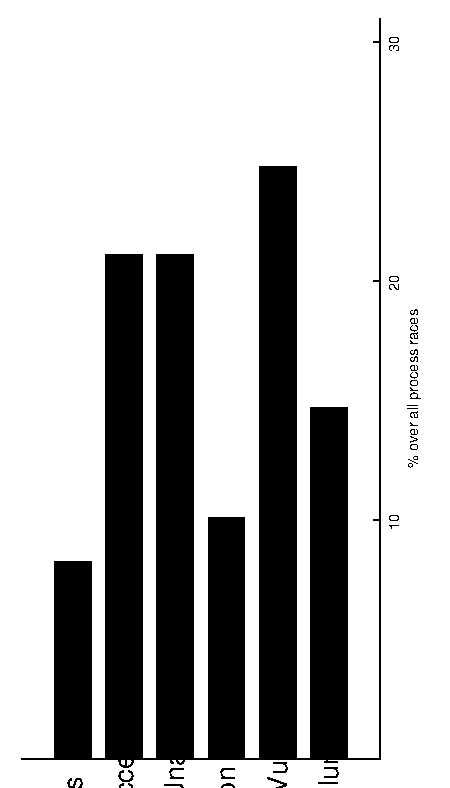
\includegraphics[width=0.45\linewidth,angle=270]{figures/racepro/race-effects}
  \caption{{\bf Process Races Breakdown by Effects.}}
  \label{racepro:fig:effects}
\end{figure}

\begin{figure}[t]
\centering
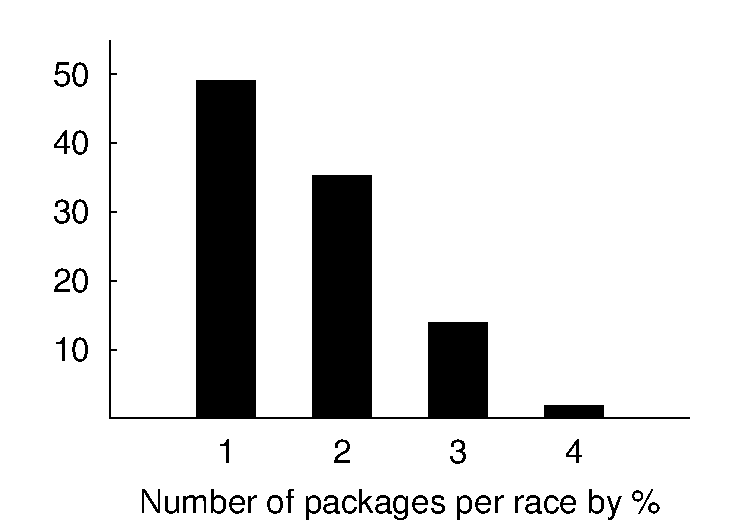
\includegraphics[width=.45\linewidth]{figures/racepro/race-packages}
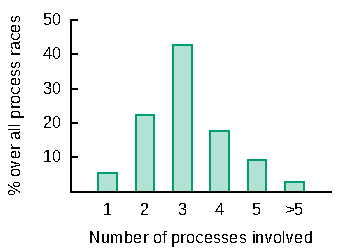
\includegraphics[width=.45\linewidth]{figures/racepro/race-processes}
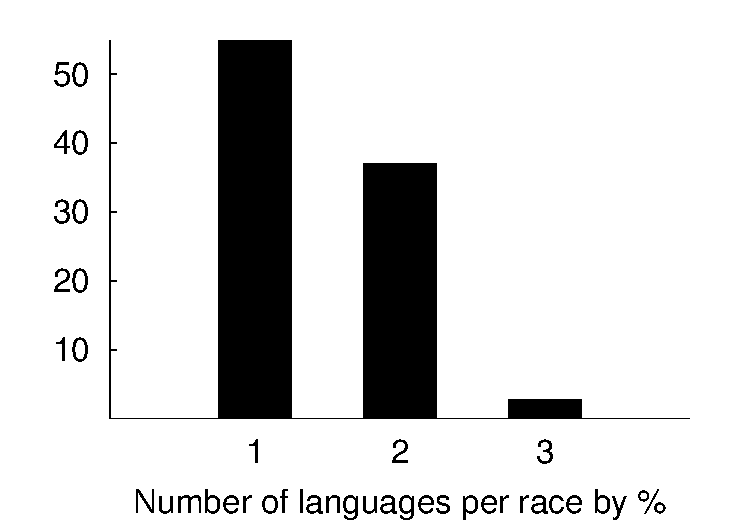
\includegraphics[width=.45\linewidth]{figures/racepro/race-languages}
\caption{{\bf Process Races Breakdown.} X axis shows the number of software
  packages, processes, or programming languages involved.  Y axis shows
  the percentage of process races that involve the specific number of
  packages, processes, or languages.  To avoid inflating the number of
  processes, we count a run of a shell script as one process.  (Each external
  command in a script causes a \code{fork}.)} \label{racepro:fig:breakdown}
\end{figure}

\para{Process races are dangerous.}  Compared to thread races that
typically corrupt volatile application memory, process races
are arguably more dangerous because they often corrupt persistent and system resources.
Indeed, the sampled process races caused security breaches, files and databases to
become corrupted, programs to read garbage, and processes to get stuck
in infinite loops. Figure~\ref{racepro:fig:effects} summarizes the effects of
all process races from Table~\ref{racepro:tab:data}.

\para{Process races are heterogeneous.}  The sampled process races
spread across over 200 programs, ranging from server
applications such as MySQL, to desktop applications such as OpenOffice,
to shell scripts in Upstart~\cite{upstart}, an event-driven
replacement of System V \code{init} scripts.  Figure~\ref{racepro:fig:breakdown}
breaks down the process races by packages, processes, and
programming languages involved.  Over half of the \nprace process races,
including all examples described in \S\ref{racepro:sec:example}, require 
interactions of at least two programs.  These programs are written in
different programming languages such as C, Java, PHP, and shell scripts,
run in multiple processes, synchronize via \code{fork} and \code{wait},
pipes, sockets, and signals, and access resources such as files, devices,
process status, and mount points.

This heterogeneity makes it difficult to apply existing detection methods
for thread races or \toctou races to process races.  For instance, static thread
race detectors~\cite{racerx:sosp03} work only with one program
written in one language, and dynamic thread race
detectors~\cite{yu:racetrack:sosp} work only with one process.  To
handle this heterogeneity, \racepro's race detection should be
system-wide. 

\para{Process races are highly elusive.} Many of the process races,
including Bug 1 and 3 described in
\S\ref{racepro:sec:example}, occur only due to site-specific software,
hardware, and user configurations.  Moreover, many of the sampled
process races, including all of those described in
\S\ref{racepro:sec:example}, occur only due to rare runtime factors. For
example, Bug 1 only occurs when a database shutdown takes longer 
than usual, and Bug 2 only occurs when a signal is delivered right 
after a child process exited.
These bugs illustrate the advantage of checking deployed systems, so that
we can rely on real users to create the diverse configurations and
executions to check.

\para{Process race patterns.}  Classified by the causes, the
\nprace process races fall into two categories.  Over two
thirds (\norder) are execution order
violations~\cite{lu:concurrency-bugs}, 
such as Bug 1, 3, and 4 in \S\ref{racepro:sec:example},
where a set of events are
supposed to occur in a fixed order, but no synchronization operations
enforce the order.
Less than one third (\natomic) are atomicity violations, including all
\toctou bugs; most of them are the simplest load-store
races, such as Bug 2 in \S\ref{racepro:sec:example}. 
Few programs we studied use standard locks (\eg, \code{flock}) to
synchronize file system accesses among processes.
These patterns suggest that a lockset-based race detection algorithm is
unlikely to work well for detecting process races.  Moreover, it is crucial
to use an algorithm that can detect order violations.

\subsection{Process Race Examples} \label{racepro:sec:example}

\begin{figure}
\centering
\begin{minipage}{.4\textwidth}
  \begin{rbox}
\begin{lstlisting}[language=C,framexleftmargin=5pt]
child = fork()
setjmp(loc)
p = wait(...) [blocks...]
...          // child exits
p = wait(...) [...returns]
...          // signaled
longjmp(loc)
p = wait(...) // error (no child)
\end{lstlisting}
\end{rbox}
\vspace{-1.5em}
  \caption{{\bf dash-MySQL Race.}}
  \label{racepro:fig:dash-mysql}
\end{minipage}
\hspace{3em}
\begin{minipage}{.4\textwidth}
  \begin{rbox}
\begin{lstlisting}[language=C,framexleftmargin=5pt]
fd = open(H,RDONLY);
read(fd, buf, ...);
close(fd);
... // update buf
... // do work
fd = open(H,WRONLY|TRUNC);
write(fd, buf, ...);
close(fd);
\end{lstlisting}
\end{rbox}
\vspace{-1.5em}
      \caption{{\bf bash Race.}}
      \label{racepro:fig:bash}
\end{minipage}
\end{figure}

\para{Bug 1: Upstart-MySQL.}  \code{mysqld} does not cleanly terminate
during system shutdown, and the file system becomes corrupted.  This
failure is due to an execution order violation where \code{S20sendsigs},
the shutdown script that terminates processes, does not wait long
enough for MySQL to cleanly shutdown. The script then fails to unmount
the file system which is still in use, so it proceeds to reboot the
system without cleanly unmounting the file system.  Its occurrence
requires a combination of many factors, including the mixed use of
Systems V initialization scripts and Upstart, a misconfiguration so
that \code{S20sendsigs} does not wait for daemons started by Upstart,
insufficient dependencies specified in MySQL's Upstart configuration
file, and a large MySQL database that takes a long time to shut down.

\para{Bug 2: dash-MySQL.} The shell wrapper
\code{mysql\_safe} of the MySQL server daemon \code{mysqld} goes into an
infinite loop with 100\% CPU usage after a MySQL update.
This failure is due to an atomicity violation in \code{dash},
a small shell Debian uses to run daemons~\cite{dash}.  It occurs
when \code{dash} is interrupted by a signal unexpectedly.
Figure~\ref{racepro:fig:dash-mysql} shows the event sequence causing this race.
To run a new background job, \code{dash} forks a child process and
adds it to the job list of \code{dash}.  It then calls \code{setjmp} to save an execution
context and waits for the child to exit.  After the child exits,
\code{wait} returns, and \code{dash} is supposed to remove the child from
the job list.  However, if a signal is delivered at this time, \code{dash}'s
signal handler will call \code{longjmp} to go back to the saved 
context, and the subsequent \code{wait} call will fail because the child's
exit status has been collected by the previous \code{wait} call.  
The job list is still not empty, so \code{dash} gets stuck waiting for the
nonexistent child to exit.  Although this bug is in \code{dash}, it is
triggered in practice by a combination of \code{dash}, the \code{mysql\_safe}
wrapper, and \code{mysqld}.

\para{Bug 3: Mutt-OpenOffice.}  OpenOffice displays
garbage when a user tries to open a Microsoft (MS) Word attachment in the
Mutt mail client.
This failure is due to an execution order violation
when \code{mutt} prematurely overwrites the contents of a file
before OpenOffice uses this file.  It involves a
combination of Mutt, OpenOffice, a user configuration entry
in Mutt, and the \code{openoffice} shell script wrapper.  The user
first configures Mutt to use the \code{openoffice} wrapper to open
MS Word attachments.  To show an attachment, \code{mutt} saves the
attachment to a temporary file, spawns the configured viewer in a new
process, and waits for the viewer process to exit.  The \code{openoffice}
wrapper spawns the actual OpenOffice binary and exits at once.
\code{mutt} mistakes this exit as the termination of the actual viewer, and
overwrites the temporary file holding the attachment with all zeros,
presumably for privacy reasons.

\para{Bug 4: bash.} The \code{bash} shell history is corrupted.
This failure is due to an atomicity violation
when multiple \code{bash} shells write concurrently
to \code{.bash\_history} without synchronization.
When \code{bash} appends to the history file, it correctly uses
\code{O\_APPEND}.  However, it also occasionally reads back the history
file and overwrites it, presumably to keep the history file under a
user-specified size.  Figure~\ref{racepro:fig:bash} shows this problematic
sequence of system calls.  \code{bash} also runs this sequence when it
exits.  When multiple \code{bash} processes exit at the same time, the
history file may be corrupted. 

\section{Architecture Overview} \label{racepro:sec:overview}


\begin{figure}[]
  \centering
  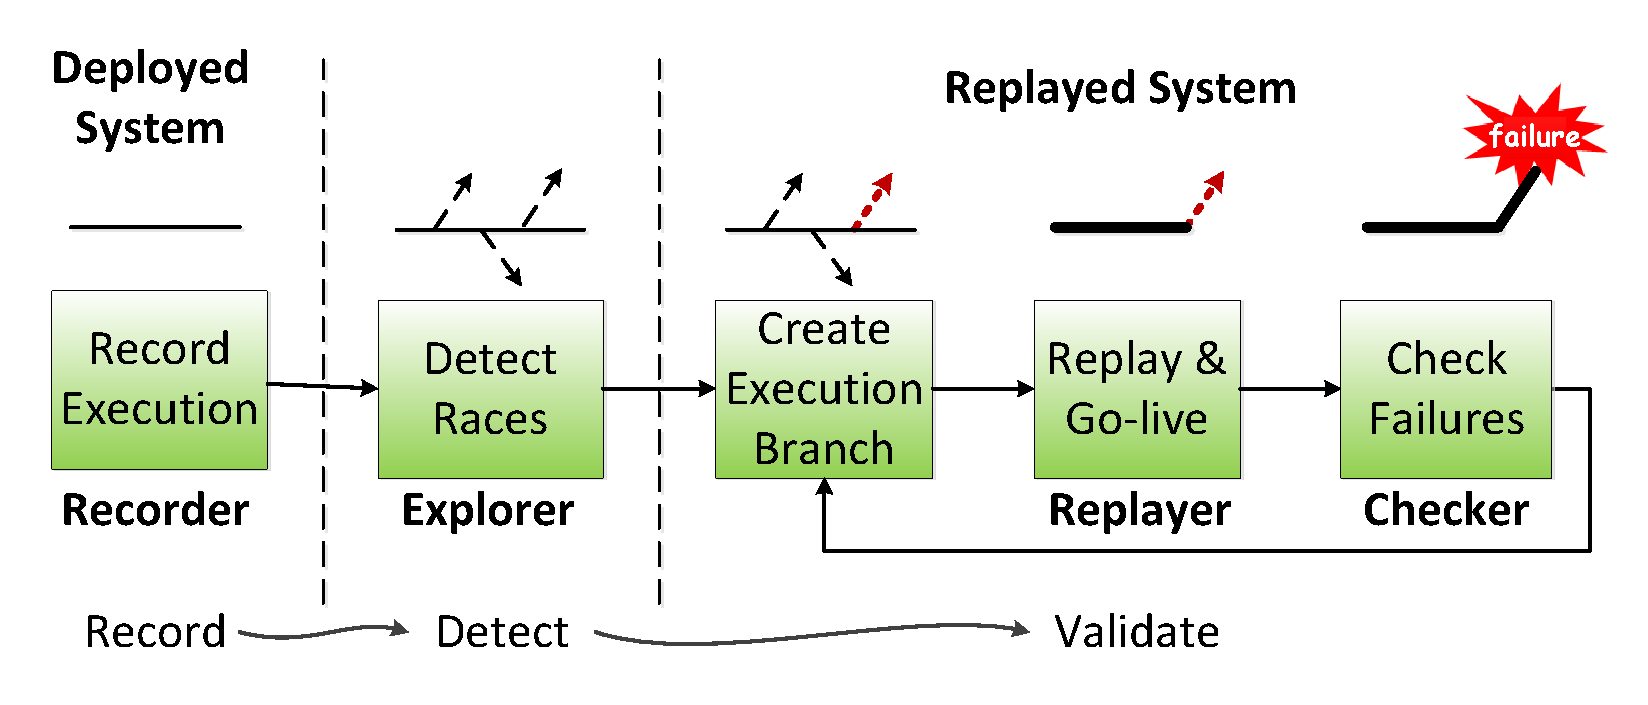
\includegraphics[width=0.9\linewidth]{figures/racepro/flow}
  \caption{{\bf \racepro Workflow.} Thin solid lines represent recorded
    executions; thick solid lines represent replayed executions.  Dashed
    arrows represent potentially buggy execution branches. The dotted
    thick arrow represents the branch \racepro selects to
    explore.} \label{racepro:fig:flow}
\end{figure}

\begin{figure}[]
  \centering
  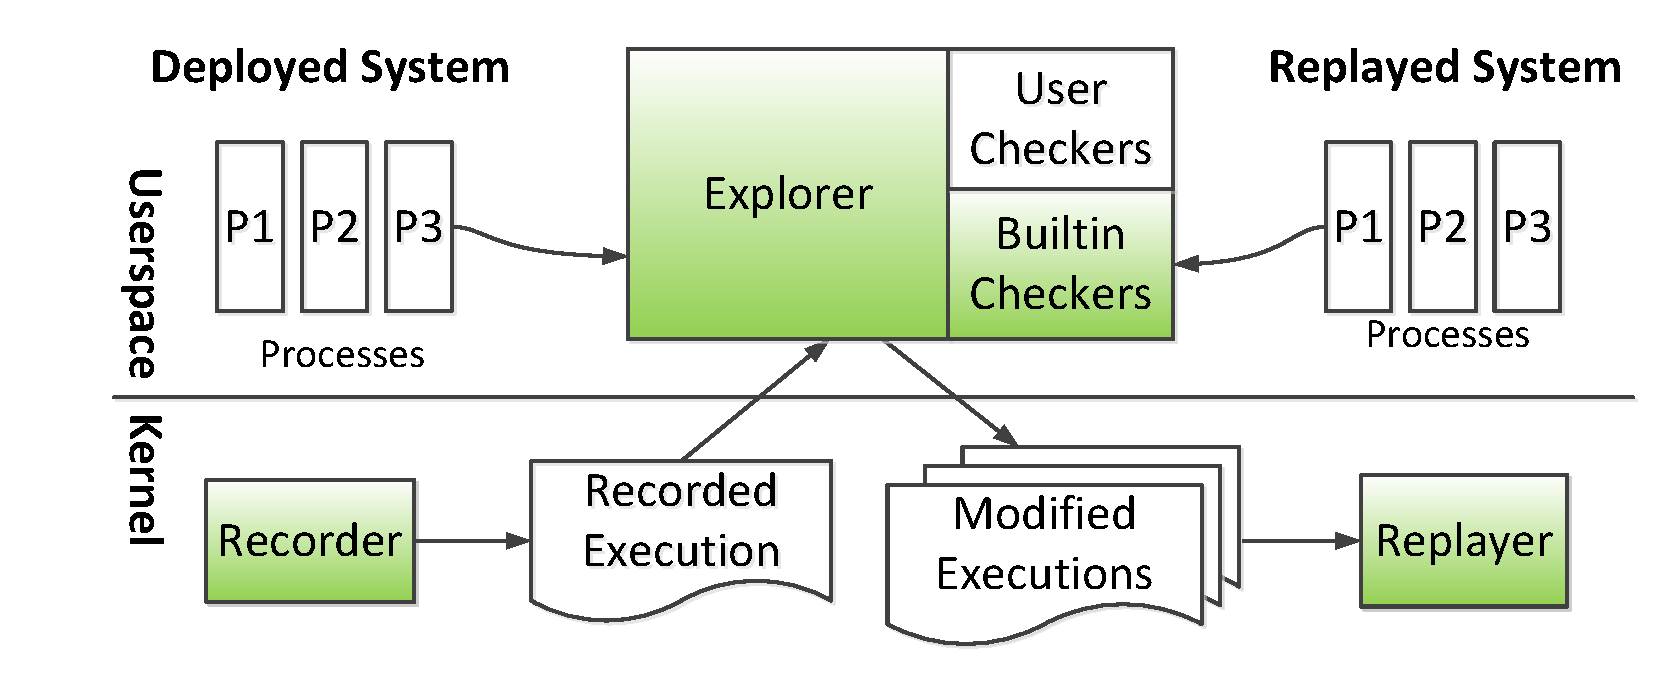
\includegraphics[width=0.9\linewidth]{figures/racepro/arch}
  \caption{{\bf \racepro Architecture.} Components are shaded. The recorder
    and the replayer run in kernel-space, and the explorer and the
    checkers run in user-space.  Recorded executions and modified
    executions are stored in files.} \label{racepro:fig:arch}
\end{figure}


\racepro is designed to automatically detect process races using the
workflow shown in Figure~\ref{racepro:fig:flow}.  
It consists of three steps,
the first of which runs on the deployed system, while the latter two can run
elsewhere on a separate replay system to avoid any performance
impact on the deployed system.
First, a \emph{recorder} records the execution of a deployed system
while the system is running and stores the recording in a log file.  Second,
an \emph{explorer} reads the log and detects load-store and wait-wakeup races
in the recorded execution.  Third, each race is validated to determine if
it is harmful.  An execution branch of the recorded execution
corresponding to each race is computed by systematically changing the
order of system calls involved in the race.  For each
execution branch, a modified log is constructed that is used to replay 
execution with the changed order of system calls.  A 
\emph{replayer} replays the respective modified log up to the
occurrence of the race, then causes it to resume live execution from
that point onward.  A set of built-in and user-provided \emph{checkers}
then check whether the execution results in misbehavior or a failure
such as a segmentation fault.  By examining the effects of a live
execution, we distinguish harmful races from false or benign ones,
thus reducing false
positives~\cite{pinsel:pldi07,racefuzzer:pldi08}. The live part 
of the re-execution is also recorded, so that users can
deterministically replay detected bugs for debugging.

Figure~\ref{racepro:fig:arch} shows the \racepro architecture used to support its
workflow.  Of the four main architectural components, the recorder
and the replayer run in kernel-space, and the explorer and checkers
run in user-space.  We will describe how \racepro records executions
(\S\ref{racepro:sec:record}) and detects (\S\ref{racepro:sec:detect}) and validates
(\S\ref{racepro:sec:validate}) races using these components.  

\section{Recording Executions} \label{racepro:sec:record}

\racepro's record-replay functionality builds on our previous work on
lightweight OS-level deterministic replay on
multiprocessors~\cite{scribe:sigmetrics10}.  This approach provides four key
benefits for detecting process races.  First, \racepro's recorder can 
record the execution of multiple processes and threads with low overhead
on a deployed system so that the replayer can later deterministically
replay that execution.  This makes \racepro's \emph{in-vivo} checking approach
possible by minimizing the performance impact of recording deployed
systems.  Second, \racepro's record-replay is application-transparent; it
does not require changing, relinking, or recompiling applications or
libraries. This enables \racepro to detect process races that are
extremely heterogeneous involving many different programs written in
different program languages.  Third, \racepro's recorder operates at the
OS level to log sufficiently fine-grained accesses to shared kernel
objects so that \racepro's explorer can detect races regardless of
high-level program semantics~(\S\ref{racepro:sec:detect}).  Finally, \racepro's
record-replay records executions such that it can later transition 
from controlled replay of the recording to live execution at any
point.  This enables \racepro to distinguish harmful races from benign
ones by allowing checkers to monitor an application for
failures~(\S\ref{racepro:sec:reexec}). 

To record the execution of multiprocess and multithreaded
applications, \racepro records all nondeterministic interactions between
applications and the OS and saves the recording as a log file.  We
highlight how key interactions involving system calls, signals, and
shared memory are handled.

\para{System calls.}  Unlike previous
work~\cite{r2:osdi,srinivasan:flashback} that records and replays a total
order of system calls, \racepro records and replays a partial order of system
calls for speed.  \racepro enforces no ordering constraints among system
calls during record-replay unless they access the same kernel object
and at least one of them modifies it, such as a \code{write} and a
\code{read} on the same file.  In that case, \racepro records the order in
the kernel in which the object is accessed by the system calls and
later replays the exact same order of accesses.  This is done by 
piggybacking on the synchronization code that the kernel already has
for serializing accesses to shared objects.  These tracked accesses
also help detect process races in a recorded execution
(\S\ref{racepro:sec:detect}). 

Table~\ref{racepro:tab:resources} lists the kernel objects tracked by \racepro.
Most of the entries correspond one-to-one to specific low-level kernel
resources, including inodes, files, file-tables, memory maps, and
process credentials. The global entry corresponds to system-wide
kernel objects, such as the hostname, file system mounts, system time,
and network interfaces. For each such system-wide resource there
is a unique global kernel object used to track accesses to that
resource. The last two entries in the table, pid and ppid, provide a
synchronization point to track dependencies on process states. For
example, the pid entry of a process is used to track instances where
the process is referenced by another process, \eg, through a system
call that references the process ID or through the \code{/proc} file
system. The ppid entry is used to track when an orphan process is
re-parented, which is visible through the \code{getppid} system call.
Both pid and ppid correspond to identifiers that are visible to
processes but cannot be modified explicitly by processes.

\begin{table}[t]
\centering
\begin{tabular}{ll}
  \toprule
{\bf Object} & {\bf Description} \\ \midrule
inode       & file, directory, socket, pipe, tty, pty, device \\
file        & file handle of an open file \\
file-table  & process file table \\
mmap        & process memory map \\
cred        & process credentials and capabilities, \eg, user ID \\
global      & system-wide properties (\eg, hostname, mounts) \\
pid         & process ID (access to process and \code{/proc}) \\
ppid        & parent process ID (synchronize \code{exit/getppid}) \\
  \bottomrule
\end{tabular}
\caption{{\bf Shared Kernel Objects Tracked.}} \label{racepro:tab:resources}
\end{table}

The recorder only tracks kernel objects whose state is visible
to user-space processes, either directly or indirectly.  For example,
inode state is accessible via the system call \code{lstat}, and
file-table state is visible through resolving of file descriptor in
many system calls. \racepro does not track accesses to kernel
objects which are entirely invisible to user-space.
This avoids tracking superfluous
accesses that may pollute the race detection results with unnecessary
dependencies.
For example, both the \code{fork} and \code{exit} system calls access the
kernel process table, but the order is unimportant to user-space. It
only matters that the lifespan of processes is observed correctly, 
which is already tracked and enforced via the pid resource.  If \racepro
tracked accesses to the kernel process table, it would mistakenly
conclude that every two \code{fork} system calls are ``racy'' because they
all modify a common resource~(\S\ref{racepro:sec:detect}).  One complication 
with this approach is that if the kernel object in question controls
assignment of identifiers (\eg, process ID in the \code{fork} example),
it may assign different identifiers during replay because the original
order of accesses is not enforced. To address this problem, \racepro
virtualizes identifiers such as process IDs to ensure the same values
are allocated during replay as in the recording.

\para{Signals.}
Deterministically replaying signals is hard since they must be
delivered at the exact same instruction in the target execution flow
as during recording.  To address this problem,
\racepro uses \emph{sync points} that correspond to synchronous kernel entries
such as system calls.  Sending 
a signal to a target process may occur at any time during the target
process's execution.  However, \racepro defers signal delivery until sync
points occur to make their timing deterministic so they are easier to
record and replay efficiently.  Unlike previous approaches, sync
points do not require hardware counters or application modifications,
and do not adversely impact application performance because they occur
frequently enough in real server and desktop applications due to OS
activities.  

\para{Shared memory.}
\racepro combines page ownership with sync points to
deterministically record and replay the order of shared memory
accesses among processes and threads.  Each shared memory page is
assigned an owner process or thread for some time interval.  The owner
can exclusively modify that page during the interval and treat it like 
private memory, avoiding the need to track all memory accesses during such
ownership periods.  Transitioning page ownership from one process or
thread to another is done using a concurrent read, exclusive write
(CREW) protocol~\cite{smp-revirt,instant-replay}.  To ensure
that ownership transitions occur at precisely the same location 
in the execution during both record and replay, \racepro defers such
transitions until the owner reaches a sync point.  When a process
tries to access an owned page, it triggers a page fault, notifies the owner,
and blocks until access is granted.  Conversely, each owner checks for
pending requests at every sync point and, if necessary, gives up 
ownership.   Page faults due to the memory interleaving under
the CREW protocol are synchronous kernel entries that
deterministically occur on replay and hence are also used as sync 
points. 

\section{Detecting Process Races} \label{racepro:sec:detect}

\racepro flags a set of system calls as a race if (1)~they are
\emph{concurrent} and therefore could have executed in a different
order than the order recorded, (2)~they access a common resource
such that reordering the accesses may change the outcome of the
execution.  To determine whether a set of system calls are concurrent, 
\racepro constructs a happens-before~\cite{lamportclock} graph for the
recorded execution (\S\ref{racepro:sec:graph}).  To determine whether a set of
system calls access common resources, \racepro obtains the shared kernel
resources accessed by system calls from the log file and models the
system calls as \emph{load} and \emph{store} micro-operations
(\S\ref{racepro:sec:model}) on those resources.  \racepro then runs a set of
happens-before based race detection algorithms to detect load-store
and wait-wakeup races (\S\ref{racepro:sec:potential}).

\subsection{The Happens-Before Graph} \label{racepro:sec:graph}

We define a partial ordering on the execution of system calls called
\emph{inherent} happens-before relations.  We say that system call
$S_1$ \emph{inherently} happens-before system call $S_2$ if (1)~$S_1$
accesses some resource before $S_2$ accesses that resource, (2)~there
is a dependency such that $S_2$ would not occur or complete unless
$S_1$ completes, and (3)~the dependency must be inferable from the
system call semantics.  For example, a \code{fork} that creates a child
process inherently happens-before any system call in the child
process, and a \code{write} to a pipe inherently happens-before 
a blocking \code{read} from the pipe.  On the other hand, there is no
inherent happens-before relation between a \code{read} and subsequent 
\code{write} to the same file.

\racepro constructs the happens-before graph using only inherent
happens-before relations, as they represent the basic constraints on
the ordering of system calls.  Given a recorded
execution, \racepro constructs a happens-before graph for all recorded
system call events by considering pairs of such events.  If two events
$S_1$ and $S_2$ occur in the same process and $S_2$ is the next
system call event that occurs after $S_1$, \racepro adds a directed edge
$S_1\rightarrow S_2$ in the happens-before graph.  If two events $S_1$
and $S_2$ occur in two different processes, \racepro adds a directed edge
$S_1\rightarrow S_2$ in four cases: 

\begin{itemize}
\item $S_1$ is a \code{fork} call, and $S_2$ is the corresponding
  \code{fork} return in the child process;
\item $S_1$ is the \code{exit} of a child process, and $S_2$ is the
  corresponding \code{wait} in the parent;
\item $S_1$ is a \code{kill} call, and $S_2$ is the corresponding signal
  delivery in the target process; or
\item $S_1$ is a stream (\eg, pipe or socket) write, and $S_2$ is a
  read from the same stream and the data written and the data read
  overlap.
\end{itemize}

We say that event $S_1$ \emph{happens-before} $S_2$ with respect to a
happens-before graph iff there is a directed path from $S_1$ to
$S_2$ in the happens-before graph.  Two events are \emph{concurrent}
with respect to a happens-before graph iff neither happens before
the other. 

\racepro also computes the vector-clocks~\cite{vectorclock} for all the
system calls in the happens-before graph.  By definition, the
vector-clock of $S_1$ is earlier than the vector-clock of $S_2$ iff
$S_1$ \emph{happens-before} $S_2$ with respect to the graph, so comparing
the vector-clocks of system calls is a fast and efficient way to test
whether they are concurrent.

Our definition of inherent happens-before does not capture all
dependencies that may constrain execution ordering. It may be missing
happens-before edges that depend on the behavior of the application
but cannot be directly inferred from the semantics of the system calls
involved. For example, the graph does not capture dependencies between
processes via shared memory. It also does not capture dependencies
caused by contents written to and read from files. For example, one
can implement a fork-join primitive using read and write operations on
a file.  In some cases, such inaccuracies may make \racepro more
conservative in flagging racy system calls and thereby identify
impossible races.  However, such cases will be filtered later by
\racepro's validation step (\S\ref{racepro:sec:validate}) and will not be reported.

\begin{figure}[]
\centering
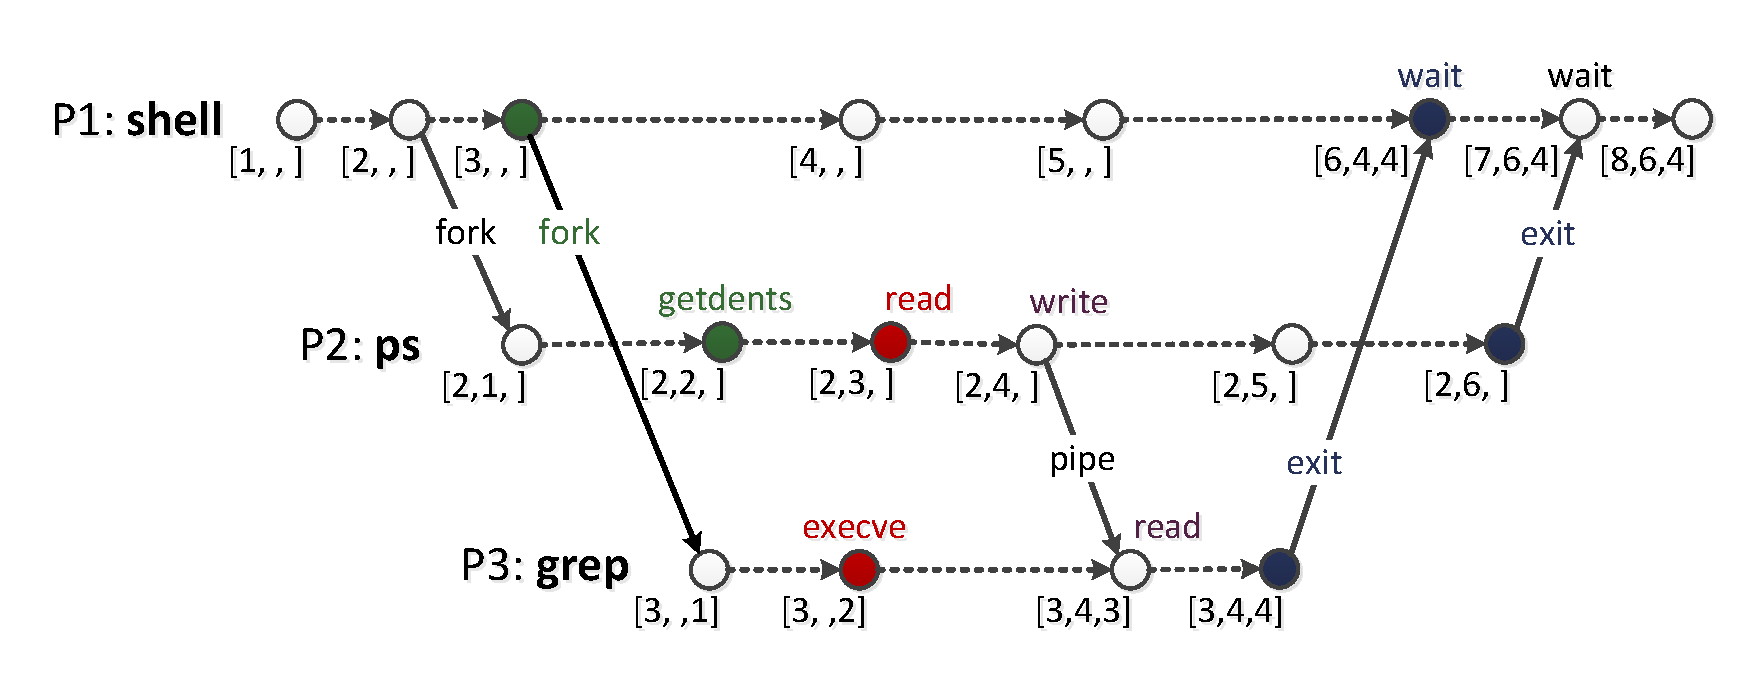
\includegraphics[width=\linewidth]{figures/racepro/psgrep}
\caption{{\bf The Happens-Before Graph for \code{ps | grep X}.}
  $P_{i=1,2,3}$ represent the processes involved.
  $[i,j,k]$ represent vector-clocks.
  The \code{read} of process $P_2$ and the \code{execve} of
  $P_3$ form a load-store race~(\S\ref{racepro:sec:load-store}), and so do the
  second \code{fork} of $P_1$ and the \code{getdents} (read directory entries) of $P_2$. The first
  \code{wait} of $P_1$ and the \code{exit}s of $P_2$ and $P_3$ form a
  wait-wakeups race~(\S\ref{racepro:sec:wait-wakeup}). For clarity, not all
  system calls are shown.} \label{racepro:fig:psgrep}
\end{figure}

Figure~\ref{racepro:fig:psgrep} shows the happens-before graph for the example
command \code{ps | grep X}.  This command creates two child processes
that access \code{grep}'s entry in the \code{/proc} directory: the process
that runs \code{grep} modifies its command-line data when executed, and
the process that runs \code{ps} reads that data.  A race exists because
both processes access the common resource in an arbitrary order, and
the end result can be either $N$ or $N+1$ lines depending on that order.

Consider the \code{execve} system call in process $P_3$ and the
\code{read} system call in process $P_2$. These two system calls are
concurrent because there is no directed path between them in the
graph. They both access a shared resource, namely, the inode of the
file \code{cmd\_line} in the directory corresponding to $P_3$ in
\code{/proc}.  Therefore, these system calls are racy: depending on the
precise execution order, \code{read} may or may not observe the new
command line with the string ``X''. Similarly, the second \code{fork}
in process $P_1$ and the \code{getdents} in process $P_3$ are also racy: 
\code{getdents} may or may not observe the newly created entry for
process $P_3$ in the \code{/proc} directory.

In contrast, consider the pipe between $P_2$ and $P_3$. This pipe is a
shared resource accessed by their \code{write} and \code{read} system calls,
respectively.  However, these two system calls are not racy because
they are not concurrent.  There exists a happens-before edge in the
graph because a read from the pipe will block until data is available
after a write to it.

\subsection{Modeling Effects of System Calls} \label{racepro:sec:model}

Existing algorithms for detecting memory races among threads rely on
identifying concurrent load and store instructions to shared memory.
To leverage such race detection algorithms, \racepro models the effects of
a system call on the kernel objects that it may access using two
micro-operations: \emph{load} and \emph{store}. These micro-operations
are analogous to the traditional load and store instructions that are
well-understood by the existing algorithms, except our micro-operations
refer to shared kernel objects, such as inodes and memory maps,
instead of an application's real shared memory.

More formally, we associate an abstract memory range with each kernel
object.  The effect of a system call on a kernel object depends on
its semantics. If the system call only observes the object's state, we
use a \emph{load(obj,range)} operation. If it may also modify the
object's state, we use a \emph{store(obj,range)} operation.  The
argument \emph{obj} indicates the affected kernel object, and the
argument \emph{range} indicates the ranges being accessed within that
object's abstract memory. A single system call may access multiple
kernel objects or even the same kernel object multiple times within
the course of its execution. 

We use a memory range for a shared kernel object instead of a single
memory location because system calls often access different
properties of an object or ranges of the object data.
For instance, \code{lstat} reads the
meta-data of files, while \code{write} writes the contents of files.
They access a common object, but because they access distinct
properties of that object, we do not consider them to race.  Likewise, 
\code{read} and \code{write} system calls to non-overlapping regions in
the same file do not race.

Memory ranges are particularly useful to model pathnames. 
Pathname creation and deletion change the parent directory structure
and may race with reading its contents, but pathname
creation, deletion, and lookup may only race with each other if given
the same pathname.  For example, both \code{creat(/tmp/a)} and
\code{unlink(/tmp/b)} may race with a \code{getdents} on \code{/tmp},
but are unrelated to each other or to an \code{lstat(/tmp/c)}. 
Modeling all pathname accesses using a single location on the parent
directory's inode is too restrictive.  Instead, we assign a unique
memory location in the parent directory's inode for each possible
pathname.  We then model pathname creation and deletion system calls 
as stores to the designated location, pathname lookup system calls as
loads from that location, and read directory system calls as loads
from the entire pathname space under that directory.

Memory ranges are also useful to model \emph{wait system calls} which
may block on events and \emph{wakeup system calls} which may trigger
events.  Example wait and wakeup system calls include \code{wait} and
\code{exit}, respectively, and a blocking \code{read} from a pipe and a
\code{write} to the pipe, respectively.
To model the effect of wait and wakeup system calls, we use a special
location in the abstract memory of the resource involved.  Wait system
calls are modeled as \emph{loads} from that location, and wakeup system
calls are modeled as \emph{stores} to that location.  For instance, the
\code{exit} system call does a \emph{store} to the special location
associated with the parent process ID, and the \code{getppid} system
call does a \emph{load} from the same location.

\begin{table}
\centering
\small
\begin{tabular}{ccl}
  \toprule
  {\bf Syscall}                    & {\bf Micro-Op} & {\bf Kernel Object}               \\ \midrule
  \multirow{5}{*}{\code{open}}     & \emph{store}   & file-table                        \\
                                   & \emph{load}    & inodes of path components         \\
                                   & \emph{store}   & inode of directory, if O\_CREAT   \\
                                   & \emph{load}    & inode of file, if no O\_CREAT     \\
                                   & \emph{store}   & data of file (range), if O\_TRUNC \\ \midrule
  \multirow{4}{*}{\code{write}}    & \emph{load}    & process file-table                \\
                                   & \emph{store}   & file handle of file               \\
                                   & \emph{store}   & inode of file                     \\
                                   & \emph{store}   & data of file (range)              \\ \midrule
  \multirow{5}{*}{\code{read}}     & \emph{load}    & process file-table                \\
                                   & \emph{store}   & file handle of file               \\
                                   & \emph{load}    & inode of file, if regular file    \\
                                   & \emph{store}   & inode of file, if a stream        \\
                                   & \emph{load}    & data of file (range)              \\ \midrule
  \multirow{4}{*}{\code{getdents}} & \emph{load}    & process file-table                \\
                                   & \emph{store}   & file handle of directory          \\
                                   & \emph{load}    & inode of directory                \\
                                   & \emph{load}    & data of directory (range)         \\ \midrule
  \multirow{3}{*}{\code{execve}}   & \emph{load}    & inodes of path components         \\
                                   & \emph{store}   & data of \code{/proc/self/status}  \\
                                   & \emph{store}   & data of \code{/proc/self/cmdline} \\ \midrule
  \multirow{2}{*}{\code{clone}}    & \emph{load}    & process memory map                \\
                                   & \emph{store}   & data of \code{/proc} directory    \\ \midrule
  \multirow{2}{*}{\code{exit}}     & \emph{store}   & 'pid' of self                     \\
                                   & \emph{store}   & 'ppid' of re-parented children    \\ \midrule
  \multirow{2}{*}{\code{wait}}     & \emph{store}   & data of \code{/proc} directory    \\
                                   & \emph{load}    & 'pid' of reaped child             \\ \midrule
  \multirow{1}{*}{\code{getppid}}  & \emph{load}    & 'ppid' of self                    \\
  \bottomrule
\end{tabular}
\caption{{\bf Micro-Operations of Common System Calls.}}
\label{racepro:tab:syscall-effects}
\end{table}

Table~\ref{racepro:tab:syscall-effects} shows the template of micro-operations
that \racepro uses to model nine common system calls: \code{open}, \code{write},
\code{read}, \code{getdents}, \code{execve}, \code{clone}
(fork a process), \code{exit}, \code{wait}, and \code{getppid}. The \code{open} system
call accesses several resources.  It stores to the process file-table to
allocate a new file descriptor, loads from the inodes of the directories
corresponding to the path components, stores to the inode of the parent
directory if the file is being created or loads from the file's inode
otherwise, and stores to the entire data range of the inode if
the file is being truncated.

The \code{write}, \code{read}, and \code{getdents} system calls access three
resources:  process file-table, file handle, and inode.  \code{write}
loads from the process file-table to locate the file handle, stores to
the file handle to update the file position, stores to the meta-data
of the file's inode in the file system, and stores to the affected
data range of the file's inode.  The last two micro-operations both
affect the file's inode, but at different offsets.  \code{read} from a
regular file and \code{getdents} are similar to \code{write}, except that
they load from the respective file's or directory's inode.  \code{read}
from a stream, such as a socket or a pipe, is also similar, except
that it consumes data and thus modifies the inode's state, so it is
modeled as a store to the corresponding inode.

The \code{execve} system call accesses several resources. It loads from
the inodes of the directories corresponding to the path components. It
also stores to the inodes of the \code{status} and \code{cmdline} files in
the \code{/proc} directory entry of the process, to reflect the newly
executed program name and command line.

The \code{clone}, \code{exit}, and \code{wait} system calls access two
resources.  \code{clone} loads from the process's memory map to create a
copy for the newborn child, and stores to the \code{/proc} directory
inode to reflect the existence of a new entry in it. \code{exit} stores
to the pid resource of the current process to set the zombie state, and
stores to the ppid resource of its children to reparent them to init.
\code{wait} stores to the reaped child's pid resource to change its state
from zombie to dead, and stores to the \code{/proc} directory inode to
remove the reaped child's entry.  \racepro detects races between 
\code{exit} and \code{wait} based on accesses to the exiting child's pid
resource.  Similarly, \code{getppid} loads from the current process's
ppid resource, and \racepro detects races between \code{exit} and \code{getppid}
based on accesses to the ppid resource.

To account for system calls that operate on streams of data, such as
reads and writes on pipes and sockets, we maintain a virtual
write-offset and read-offset for such resources.  These offsets are
advanced in response to write and read operations, respectively.
Consider a 
stream object with write-offset $L_W$ and read-offset $L_R$. A
\code{write(fd,buf,n)} is modeled as a \emph{store} to the memory range
$[L_W..L_W+n]$ of the object, and also advances $L_W$ by $n$. A 
\code{read(fd,buf,n)} is modeled as a \emph{load} from the memory range
$[L_R..L_R+\tilde{n}]$, where $\tilde{n} = min(L_W-L_R,n)$, and also 
advances $L_R$ by $\tilde{n}$.

To account for the effects of signal delivery and handling, we
model signals in a way that reflects the possibility of a signal to
affect any system call, not just the one system call that was actually
affected in the recording.  We associate a unique abstract memory  
location with each signal. A \code{kill} system call that sends a signal
is modeled as a \emph{store} to this location. Each system call in
the target process is considered to access that location, and
therefore modeled as a \emph{load} from all the signals. This method 
ensures that any system call that may be affected by a signal would
access the shared object that represents that signal.

\subsection{Race Detection Algorithms} \label{racepro:sec:potential}

Building on the happens-before graph and the modeling of system calls
as micro-operations, \racepro detects three types of process races:
load-store races (\S\ref{racepro:sec:load-store}), wait-wakeups races
(\S\ref{racepro:sec:wait-wakeup}), and wakeup-waits races
(\S\ref{racepro:sec:wakeup-wait}).  \racepro may also be extended to detect
other types of races (\S\ref{racepro:sec:multilevel}).

\paragraph{Load-Store Races} \label{racepro:sec:load-store}

A load-store race occurs when two system calls concurrently access the
same shared object and at least one is a \emph{store} operation. In this
case, the two system calls could have executed in the reverse order.
\racepro flags two system calls as a load-store race if (1)~they are
concurrent; (2)~they access the same shared kernel object, and (3)~at
least one access is a \emph{store}. In the \code{ps | grep X}
example shown in Figure~\ref{racepro:fig:psgrep}, the system calls
\code{read} and \code{execve} are flagged as a race because they are
concurrent, they access the same resource, and at least one,
\code{execve}, does a \emph{store}. In contrast, the system call 
\code{exit} of $P_3$ also stores to the same resource, but is not
flagged as a race because it is not concurrent with any of them as 
\code{read} happens-before \code{exit} and \code{execve} happens-before
\code{exit}. 

\racepro detects load-store races using a straightforward happens-before-based
race detection algorithm. We chose a happens-before over
lockset because processes rarely use standard locks (\S\ref{racepro:sec:study}). 
\racepro iterates through all the shared kernel objects in the
recording.  For each shared object, it considers the set of all
accesses to that object by all system calls, and divides this set into
per-process lists, such that the list $L_i$ of process $P_i$ contains
all the accesses performed by that process. \racepro now looks at all
pairs of processes, $P_i$, $P_j$, $i \neq j$, and considers their
accesses to the object. For each access $S_n \in L_i$, it scans
through the accesses $S_m \in L_j$.  If the vector-clocks of $S_n$ and
$S_m$ are concurrent, the pair of system calls is marked as a race. If
$S_n \rightarrow S_m$, then $S_n \rightarrow S_{m+k}$, so the scan is
aborted and the next access $S_{n+1} \in L_i$ is considered. If $S_m
\rightarrow S_n$, then $S_m \rightarrow S_{n+k}$, so $S_{m+1} \in L_j$
is saved so that the next scan of accesses from $L_j$ will start from
$S_{m+1}$, since we know that earlier events happened-before all
remaining accesses in $L_i$.

Because system calls may access more than one shared object
during their execution, it is possible that the same pair of system
calls will be marked more than once. For example, two \code{write} system
calls from different processes to the same location in the same file
will be marked twice, once when the meta-data of the inode is
considered, and once when the data of the file is considered. Because
\racepro detects and later validates (\S\ref{racepro:sec:validate}) races at the
granularity of system calls, it only reports the respective pair of
system calls once.

\racepro may produce a myriad of races, which can take a long time to
produce and later validate.  To address this concern, \racepro prioritizes 
which races to examine in two ways. First, \racepro may defer or entirely skip
races that are less likely to prove harmful, depending on the system
calls and resource involved. For example,  when analyzing the execution
of a parallel compilation, resources related to visual output may be
skipped: although many processes may be writing to the standard
output, races, if they exist, are likely to be benign.  Second, \racepro
ranks pairs of system calls according to their distance from each
other in the happens-before graph, and examines nearer system calls
first. 

\paragraph{Wait-Wakeups Races} \label{racepro:sec:wait-wakeup}

A wait-wakeups race occurs when a wait system call may be woken up
by more than a single matching wakeup system call. 
If the wakeup system calls executed in a different order, the
wait system call could have picked a different wakeup than in the
original execution.  Wait-wakeups races involve at least three system
calls.  For instance, a \code{wait} system call which does not indicate a
specific process identifier to wait for will complete if any of its
children terminate.  Likewise, a blocking \code{read} from a stream will
complete after any \code{write} to the stream. 

In these cases, the wait system call essentially uses a 
\emph{wildcard} argument for the wakeup condition so that there can be
multiple system calls that match the wakeup condition depending on
their order of execution.  The wait-wakeups race requires a wildcard,
otherwise there is only a single matching system call, and thus a
single execution order.  For instance, a \code{wait} system call that
requests a specific process identifier must be matched by the exit of
that process. In this case, the wait-wakeup relationship implies an
inherent happens-before edge in the happens-before graph, since the
two system calls must always occur in that order.

\racepro flags three system calls as a wait-wakeups race if (1)~one is a
wait system call, (2)~the other two are wakeup system calls that match
the wait condition, and (3)~the wait system call did not happen-before
any of the wakeup system calls.
In the \code{ps | grep X} example shown in Figure~\ref{racepro:fig:psgrep},
the two \code{exit} system calls of $P_2$ and $P_3$ and the first
\code{wait} system call of $P_1$ are flagged as a wait-wakeups race since
both \code{exit} calls are concurrent and can match the \code{wait}.  In
contrast, the \code{write} and \code{read} system calls to and from the pipe
are not flagged as a race, because there does not exist a second
wakeup system call that matches the \code{read}. 

\racepro detects wait-wakeups races using an algorithm that builds on the
load-store race detection algorithm, with three main differences. First,
the algorithm considers only those accesses that correspond to wait and
wakeup system calls by looking only at locations in the abstract
memory reserved for wait and wakeup actions.  Second, it considers
only pairs of accesses where one is a \emph{load} and the other is a
\emph{store},
corresponding to one wait and one wakeup system calls. The wait system
call must not happen-before the wakeup system call. Third, for each
candidate pair of wait and wakeup system calls $S_1$ and $S_2$, \racepro
narrows its search to the remaining wakeup system calls that match the
wait system call by looking for system calls that store to the same
abstract memory location.  For each matching wakeup system call $S_3$,
\racepro checks whether it would form a wait-wakeups race together with
$S_1$ and $S_2$. 

\begin{figure}[t]
  \begin{minipage}{\linewidth}
    \centering
    \begin{minipage}{.42\linewidth}
      \begin{rbox}
        \centering
        \begin{tabular}{ccc}
                  & {\bf P1}      & {\bf P2}     \\ \hline
                  & $\cdots$      &              \\
          $S_1$:  & write(P, 10); &              \\
          $S_2$:  & write(P, 10); & $\cdots$     \\
          $S_3$:  & $\cdots$      & read(P, 20); \\
                  &               & $\cdots$     \\
        \end{tabular}
      \end{rbox}
      \vspace{-2.2em}
      \center{(a)}
    \end{minipage}
    \hspace{3em}
    \begin{minipage}{.42\linewidth}
      \begin{rbox}
        \centering
        \begin{tabular}{ccc}
                   & {\bf P1}      & {\bf P2}     \\ \hline
                   & $\cdots$      &              \\
          $S_1$:   & write(P, 10); & $\cdots$     \\
          $S_2$:   &               & read(P, 20); \\
          $S_3$:   & write(P, 10); & $\cdots$     \\
                   & $\cdots$      &              \\
        \end{tabular}
      \end{rbox}
      \vspace{-2.2em}
      \center{(b)}
    \end{minipage}
  \end{minipage}
  \caption{{\bf Wait-Wakeups Races in Streams.}}
  \label{racepro:fig:streams}
\end{figure}

The relative order of the wakeup system calls may matter if their
effect on the resource is cumulative. For instance,
Figure~\ref{racepro:fig:streams} depicts a cumulative wait-wakeups scenario
in which the order of two \code{write} system calls to the same stream
determines what a matching \code{read} would observe.  
A \code{read} from a stream may return less data than requested if the
data in the buffer is insufficient. 
In Figure~\ref{racepro:fig:streams}a, a blocking \code{read} occurs after two 
\code{write}s and consumes their cumulative data.  However, in
Figure~\ref{racepro:fig:streams}b, the \code{read} occurs before the second
\code{write} and returns the data only from the first \code{write}. 
Note that $S_2$ and $S_3$ in Figure~\ref{racepro:fig:streams}a do not form a
load-store race as $S_2$ inherently happens-before $S_3$.
Thus, \racepro flags either case as a wait-wakeups race.
The relative order of the wakeup system calls does not matter if their
effect on the resource is not cumulative, such as with \code{wait} and
\code{exit} system calls.

\paragraph{Wakeup-Waits Races} \label{racepro:sec:wakeup-wait}

A wakeup-waits race occurs when a wakeup system call may wake up
more than a single matching wait system call.
Like wait-wakeups races, wakeup-waits races
involve at least three system calls. For example, a \code{connect} system
call to a listening socket will wake up any processes which may have a
pending \code{accept} on that socket; the popular Apache Web server uses
this method to balance incoming requests.  As another example, a
signal sent to a process may interrupt the process during a system
call. Depending on the exact timing of events, the signal may be
delivered at different times and interrupt different system calls.

Some wakeup system calls only affect the first matching wait system
call that gets executed; that system call ``consumes'' the wakeup and
the remaining wait system calls must wait for a subsequent wakeup.
Examples include \code{connect} and \code{accept} system calls, and \code{read}
and \code{write} system calls on streams. In contrast, when two processes 
monitor the same file using the \code{select} system call, a file state
change will notify both processes equally. Even in this case, a race
exists as the behavior depends on which wait system calls executes
first.

\racepro flags three system calls as a wakeup-waits race if (1)~one is a
wakeup system call, (2)~the other two are wait system calls that match
the wakeup, (3)~the wait system calls did not happen-before
the wakeup system call. To detect wakeup-waits races, \racepro builds on
the wait-wakeups race detection algorithm with one difference.  For
each candidate pair of wait and wakeup system calls $S_1$ and 
$S_2$, \racepro narrows its search to the remaining wait system calls
that match the wakeup system call by looking for system calls that
load from the same abstract memory location.  For each matching wait
system call $S_3$, \racepro checks whether it would form a wakeup-waits
race together with $S_1$ and $S_2$.

\paragraph{Many-System-Calls Races} \label{racepro:sec:multilevel}

\racepro's algorithms handle races that involve two system calls for
load-store races, and three system calls for both wait-wakeups and
wakeup-waits races. However, it is also possible that a race involves
more system calls. For example, consider a load-store race that comprises
a sequence of four system calls that only if executed in the
reverse order, from last to first, will produce a bug.  \racepro's
algorithm will not detect this load-store race since it only
considers one pair of system calls at a time.  To detect such races,
the algorithms can be extended to consider more system calls at a time
and more complex patterns of races.  An alternative approach is to apply
\racepro's analysis recursively on modified executions
(\S\ref{racepro:sec:reexec}). 
\section{Validating Races}  \label{racepro:sec:validate}

A detected process race may be either benign or harmful, depending on
whether it leads to a failure.  For instance, consider the
\code{ps | grep X} example again which may output either $N$ or $N+1$
lines.  When run from the command line, this race is usually benign since
most users will automatically recognize and ignore the difference.
However, for applications that rely on one specific output, this race can
be harmful and lead to a failure (\S\ref{racepro:sec:eval}).

To avoid false positives, \racepro validates whether detected races
are harmful and reports only harmful races as bugs.  
For each race, it creates an execution branch in which the racy system
calls, which we refer to as \emph{anchor} system calls, would occur in
a different order from the original recorded
execution~(\S\ref{racepro:sec:branches}). It replays the modified 
execution until the race occurs, then makes the execution
go-live~(\S\ref{racepro:sec:reexec}).  It checks the live execution for
failures~(\S\ref{racepro:sec:check}), and, if found, reports the race as a 
bug.

\subsection{Creating Execution Branches}  \label{racepro:sec:branches}

\racepro does not replay the original recorded execution, but
instead replays an execution branch built from the original execution
in a controlled way. The execution branch is a truncated and modified
version of the original log file.  Given a detected race which, based
on its type, involves two or three anchor system calls, \racepro creates an
execution branch in two steps.  First, it copies the sequence of
log events from the original execution recording \emph{up to} the anchor
system calls.  Then, it adds the anchor system calls with suitable
ordering constraints so that they will be replayed in an order that makes
the race resolve differently than in the original recorded execution.
The rest of the log events from the original execution are not
included in the modified version.

A key requirement in the first step above is that the definition of
\emph{up to} must form a \emph{consistent cut}~\cite{vectorclock}
across all the processes to avoid deadlocks in replay.  A consistent
cut is a set of system calls, one from each process, that includes the
anchor system calls, such that all system calls and other log events
that occurred before this set are on one side of the cut.  For
instance, if $S_1$ in process $P_1$ happens-before $S_2$ in process
$P_2$ and we include $S_2$ in the consistent cut, then we must also
include $S_1$ in the cut.

To compute a consistent cut for a set of anchor system calls,
\racepro simply merges the vector-clocks of the anchor system calls into
a unified vector-clock by taking the latest clock value for each
process.  In the resulting vector-clock, the clock value for each
process indicates the last observed happens-before path from that process
to any of the anchor system calls.  By definition, the source of this
happens-before edge is also the last system call of that process that must
be included in the cut.  For instance, the unified vector-clock for the
\code{read} and \code{execve}
race in Figure~\ref{racepro:fig:psgrep} is $[3,3,2]$, and the consistent cut
includes the second \code{fork} of $P_1$, \code{read} of $P_2$, and
\code{execve} of $P_3$.

Given a consistent cut, \racepro copies the log events of each process,
except the anchor system calls, until the clock value for that process
is reached.  It then adds the anchors in a particular order.  For
load-store races, there are two anchor system calls.  To generate the
execution branch, \racepro simply flips the order of the anchors compared
to the original execution; it first adds the system call that occurred
\emph{second} in the original execution, followed by the one that
occurred \emph{first}. It also adds an ordering constraint to ensure
that they will be replayed in that order. 

For wait-wakeups races, there are three anchor system calls: two wakeup
system calls and a wait system call. To generate the execution branch,
\racepro first adds both wakeup system calls, then adds a modified version
of the wait system call in which its wildcard argument is replaced
with a specific argument that will match the wakeup system call that
was \emph{not} picked in the original execution.  For example, consider
a race with two child processes in \code{exit}, either of which may wake
up a parent process in \code{wait}.  \racepro first adds both \code{exit}
system calls, then the \code{wait} system call modified such that its
wildcard argument is replaced by a specific argument that will cause
this \code{wait} to pick the \code{exit} of the child that was
not picked in the original execution. It also adds a constraint
to ensure that the parent will execute after that child's \code{exit}.
The other child is not constrained.

For wakeup-waits races, there are also three anchor system calls: one
wakeup system call and two wait system calls. To generate the
execution branch, \racepro simply flips the order of the two wait system
calls compared to the original execution.  Races that involve signals,
which may be delivered earlier or later than in the original
execution, are handled differently.  To generate an execution branch
for a signal to be delivered earlier, \racepro simply inserts the signal
delivery event at an earlier location which is thereby considered one
of the anchors of the consistent cut.  In contrast, delivering a
signal arbitrarily later is likely to cause replay
divergence~(\S\ref{racepro:sec:reexec}).  Instead, \racepro only considers
delivering a signal later if it interrupted a system call in the
recorded execution, in which case the signal is instead delivered
promptly after the corresponding system call completes when replayed. 

Reordering of the anchor system calls may also imply reordering of
additional system calls that also access the same resources. Consider
the execution scenario depicted in Figure~\ref{racepro:fig:reorder}, which
involves three processes and five system calls that access the same
resource. The system calls $S_1$ and $S_5$ form a load-store race. To
generate the modified execution for this race, \racepro will make the
following changes: (1)~it will include $S_1$ but not $S_2$, because
system calls following the anchors remain outside the cut and are
truncated; (2)~it will reorder $S_5$, and therefore $S_4$ too, with
respect to $S_1$; and (3)~depending on the consistent cut, it will
either exclude $S_3$ or reorder $S_3$ with respect to $S_1$.
\racepro adjusts the modified recording so that it will enforce the new
partial order of system calls instead of the partial order of system
calls in the original execution.

\subsection{Replaying Execution Branches and Going Live}  \label{racepro:sec:reexec}

\racepro's replayer provides deterministic replay of the originally
recorded execution and also ensures that successful replay of a
modified execution is also deterministic.  Given a modified execution,
\racepro replays each recorded event while preserving the partial order
indicated by the recording. The last events replayed are the
anchor system calls. To force races to resolve as desired, \racepro
replays the anchor system calls serially, one by one, while holding
the remaining processes inactive.  From that point onward, it
allows the processes to go live to resume normal execution.

\para{Go Live.}
The ability to go live by resuming live execution from a replay is
fundamental for allowing \racepro to validate whether races manifest
into real bugs or not, and thereby avoid reporting false-positives.
To go live, \racepro faces two challenges.  First, \racepro
must ensure that replayed processes perceive the underlying system to
be the same as at the time of recording. For example, system
identifiers such as process IDs must remain the same for processes to
run correctly after they transition to live execution. \racepro leverages
OS virtualization to encapsulate processes in a virtual
execution environment that provides the same private, virtualized view
of the system when the session is replayed or goes live as when it was
recorded~\cite{scribe:sigmetrics10}. Processes only see virtual
identifiers that always stay the same so that the session can go live
at any time.  Second, \racepro needs to not only replay the application
state in user-space, but also the corresponding state that is
internally maintained by the operating system for the processes.  For
example, actions such as creating a pipe and writing to it must be
done as is so that the pipe exists and has suitable state should the
process transition to live execution. 

\begin{figure}[t]
  \centering
  \begin{minipage}{.55\linewidth}
    \begin{rbox}
      \centering
      \begin{tabular}{lccc}
               & {\bf P1}    & {\bf P2}    & {\bf P3}    \\ \hline
               & $\cdots$    &             &             \\
        $S_1$: & syscall(R); &             &             \\
        $S_2$: & syscall(R); &             & $\cdots$    \\
        $S_3$: & $\cdots$    & $\cdots$    & syscall(R); \\
        $S_4$: &             & syscall(R); & $\cdots$    \\
        $S_5$: &             & syscall(R); &             \\
               &             & $\cdots$    &             \\
      \end{tabular}
    \end{rbox}
  \end{minipage}
  \caption{{\bf Replay Divergence Due to Reordering.}}
  \label{racepro:fig:reorder}
\end{figure}

\racepro works best when a go-live execution requests no inputs from users or
external processes; such executions include parallel make, parallel boot,
and executions of non-interactive programs.  If a go-live execution
requests external inputs, \racepro tries to replay the inputs recorded from
the original execution.  Currently \racepro replays standard inputs from users
and pipe or socket data received from external processes.  It does not
replay data read from the file system.  Instead, it checkpoints the file
system before recording an execution and restores to this checkpoint
before each replay, using unionfs~\cite{unionfs}, which has
low overhead.  Replaying inputs may not
always work because the go-live execution differs from the original
execution, but we have not found it a problem in our evaluation because
tightly coupled processes should be recorded together anyway.

\racepro can be applied recursively to detect races involving more system
calls (\S\ref{racepro:sec:multilevel}). Since it already records the go-live
portion of modified executions, doing so is as easy as running the
same detection logic on these new recordings. This essentially turns
\racepro into a model checker~\cite{flanagan:dynamicpo}. However, we leave
this mode off by default because exhaustive model checking is quite
expensive and it is probably more desirable to spend limited checking
resources on real executions over the fake checking-generated
executions.

\para{Replay Divergence.}
\racepro's replayer may not be able to replay some execution branches due
to \emph{replay divergence}.  This can result from trying to replay a
modified recording instead of the original recording.
Replay divergence occurs when there is a mismatch between the actual
actions of a replayed process and what
is scripted in the execution recording. The mismatch could be between
the actual system call and the expected system call or, even if the
system calls match, between the resources actually accessed by the
system call and the resources expected to be accessed.  When a
divergence failure occurs for some execution branch, \racepro does not
flag the corresponding race as a bug because it lacks evidence to that
end.

Divergence is commonly caused when the reordering of the anchor system
calls implies reordering of additional system calls that also access
the same resources. Consider again the execution scenario depicted in
Figure~\ref{racepro:fig:reorder} in which the system calls $S_1$ and
$S_5$ form a load-store race and the modified execution branch
reorders the systems calls as $S_3$, $S_4$, $S_5$, and $S_1$ while
dropping $S_2$ as being outside the cut.  A replay divergence may
occur if the execution of $S_5$ depended on $S_2$ which was dropped
out, or if the execution of $S_4$ depends on $S_1$ which was reordered
with respect to $S_4$. Figure~\ref{racepro:fig:diverge}a illustrates the
former scenario.   Reordering the two \code{creat} system calls would cause
$P_2$ to call \code{unlink} before $P_1$'s \code{creat}.  The call will fail
and $P_2$ will not call \code{creat} and thus diverge from the recorded
execution. 

Divergence can also be caused when processes rely on a specific
execution ordering of system calls in a way that is not tracked by
\racepro.  Figure~\ref{racepro:fig:diverge}b illustrates one such scenario where
process $P_1$ executes system call $S_1$ to write data to a file, and
process $P_2$'s execution depends on data read from file by $S_2$. If
$P_2$ depends on the specific data written by $S_1$, then reordering
$S_1$ and $S_2$ will almost certainly cause a divergence. Were the
dependency on the file's content considered an inherent happens-before
$S_1 \rightarrow S_2$, \racepro's explorer would not have flagged the race
in the first place. However, it is prohibitively expensive, and in
some cases impossible, to track generic semantics of applications.

Another cause for divergence is use of shared memory. Recall that
shared memory accesses are tracked by the recorder and enforced by the
replayer. However, reordering of system calls may lead to reordering
of shared memory accesses as well, which will certainly lead to replay
divergence. \racepro mitigates this effect by permitting \emph{relaxed}
execution from where the reordering takes place. In this mode the
replayer does not enforce memory access ordering, but continues to
enforce other ordering constraints such as partial ordering of system
calls. This improves the chances that the replayed execution reach the
point of go-live.  However, accesses to shared memory may
now resolve arbitrarily and still cause divergence. For this reason
\racepro is likely to be less effective in finding races on OS resources
between threads of the same process.  We believe that such races are
relatively unlikely to occur.

\begin{figure}[t]
  \begin{minipage}{\linewidth}
    \centering
    \begin{minipage}{.42\linewidth}
      \begin{rbox}
        \centering
        \begin{tabular}{ccc}
                 & {\bf P1}  & {\bf P2}                                \\ \hline
                 & $\cdots$  &                                         \\
          $S_1$: & creat(F); & $\cdots$                                \\
          $S_2$: & $\cdots$  & \multicolumn{1}{l}{ r = unlink(F); }    \\
                 &           & \multicolumn{1}{l}{ {\bf if} (r == 0) } \\
          $S_3$: &           & \multicolumn{1}{l}{ ~~~~~~creat(F); }   \\
                 &           & $\cdots$                                \\
        \end{tabular}
      \end{rbox}
      \vspace{-2.2em}
      \center{(a)}
    \end{minipage}
    \hspace{3em}
    \begin{minipage}{.42\linewidth}
      \begin{rbox}
        \centering
        \begin{tabular}{ccc}
                 & {\bf P1}     & {\bf P2}                                  \\ \hline
                 & $\cdots$     &                                           \\
          $S_1$: & write(F, x); & $\cdots$                                  \\
          $S_2$: & $\cdots$     & \multicolumn{1}{l}{ read(F, b); }         \\
                 &              & \multicolumn{1}{l}{ {\bf if} (b == `x') } \\
          $S_3$: &              & \multicolumn{1}{l}{ ~~~~~~write(F, y); }  \\
                 &              & $\cdots$                                  \\
        \end{tabular}
      \end{rbox}
      \vspace{-2.2em}
      \center{(b)}
    \end{minipage}
  \end{minipage}
  \caption{{\bf Replay Divergence Examples.}}
  \label{racepro:fig:diverge}
\end{figure}

\begin{table}[t]
\small
\centering
% \setlength{\tabcolsep}{3pt}
\begin{tabular}{cp{12cm}}
  \toprule
{\bf Bug ID} & {\bf Description} \\ \midrule
debian-294579    & concurrent \code{adduser} processes read and write \code{/etc/passwd} without synchronization, corrupting this file           \\
debian-438076    & \code{mv} unlinks the target file before calling atomic \code{rename}, violating the atomicity requirement on \code{mv}       \\
debian-399930    & \code{logrotate} creates a new file then sets it writable, but deamons may observe it without write permissions               \\
redhat-54127     & \code{ps | grep} race causes a wrong version of \code{licq 7.3} to be started                                                 \\
launchpad-596064 & \code{upstart} does not wait until \code{smbd} creates a directory before spawning \code{nmbd}, which requires that directory \\
launchpad-10809  & \code{bash} updates the history file without synchronization, corrupting this file                                            \\
\midrule
new-1 & \code{tcsh 6.17} updates the history file without synchronization, even when ``savehist merge'' is set                    \\
new-2 & \code{updatedb} removes old database before renaming the new one, so \code{locate} finds nothing (\code{findutils 4.4.2}) \\
new-3 & concurrent \code{updatedb} processes may cause the database to be empty                                                   \\
new-4 & incorrect dependencies in Makefile of \code{abr2gbr 1.0.3} may causes compilation failure                                 \\
\bottomrule
\end{tabular}
\caption{{\bf Bugs Found by \racepro.}  Bugs are identified by ``distribution -
bug ID''. New bugs  are identified as ``new - bug number''}.
  \label{racepro:tab:bugs}
\end{table}

Replay divergence is reportedly a serious problem for a previous race
classifier~\cite{pinsel:pldi07}, where it can occur for two
reasons: the race being validated does occur and causes the execution
to run code or access data not recorded originally, or the race being
validated cannot occur and is a false positive. In contrast, replay
divergence actually \emph{helps} \racepro to distinguish root-cause races
from other races. By relying on a replay followed by transition to
live execution, \racepro is no longer concerned with the first scenario.
If replay diverges, \racepro can tell that the race is a false positive
and discard it.

Moreover, if the divergence is not due to untracked interactions or
shared memory discussed above (or file locking, also untracked by
\racepro), then there must exist another race that is ``tighter'' than the
one being validated. The other race may involve the same resource or a
different one. For example, in Figure~\ref{racepro:fig:diverge}b the race
between $S_1$ and $S_3$ causes divergence because of another race
between $S_1$ and $S_2$. The latter race is ``tighter'' in the sense
that $S_2$ is closer to $S_1$ because $S_2 \rightarrow S_3$; the race
between $S_1$ and $S_2$ subsumes the race between $S_1$ and $S_3$. In
other words, discarding races that cause replay divergence helps \racepro
to find root-cause races. We believe the go-live mechanism can benefit
existing replay-based thread-race classifiers.

\subsection{Checking Execution Branches}  \label{racepro:sec:check}

When the replay of an execution branch switches to live
execution, \racepro no longer controls the execution. Rather, it records
the execution from that point on, and activates a checker to monitor
the execution for failures or incorrect behavior. If the checker
detects a failure that did not occur during recording,
it reports a bug and saves the combined
execution recording, consisting of the original recording followed by
the new recording, so that users can deterministically replay it for
debugging.

\racepro provides a set of built-in checkers to detect bad application
behavior. The built-in checker can detect erroneous behavior such as
segmentation faults, infinite loops (via timeouts), error messages in
system logs, and failed commands with non-zero exit status. 
In addition, \racepro can also run system-provided checker
programs such as \code{fsck}.

Moreover, \racepro allows users to plug in domain-specific checkers. To do
so, a user need only provide a program or even a shell script that
will run concurrently along the live execution. For instance, such
scripts could compare the output produced by a modified execution to that
of the original execution, and flag significant differences as errors.
It is also possible to use existing test-suites already provided
with many application packages.  These test-suites are particularly handy if
the target application is a server. For instance, both the Apache web
server and the MySQL database server are shipped with basic though
useful test suites, which could be executed against a modified server.
Finally it may also compare the output of the go-live execution with a
linearized run~\cite{linearizable:eurosys11}.

By running checkers on live executions, \racepro guarantees that observed
failures always correspond to real executions, thus eliminating false
positives if the checkers are accurate.  Moreover, the process races \racepro
detects are often the root cause of the failures, aiding developers in
diagnosis.  In rare cases, after a modified execution goes live, it may
encounter an unrelated bug.  \racepro still provides an execution recording
useful for debugging, but without pointing out the root-cause.

As in many other checking frameworks, \racepro can detect only what is checked.
Although its built-in checkers can detect many errors
(\S\ref{racepro:sec:bug}), it may miss domain-specific ``silent''
corruptions.  Fortunately, recent work has developed techniques to check
advanced properties such as conflict serializability or
linearizability~\cite{linearizable:eurosys11}, which \racepro can leverage.

\racepro may have false negatives.  A main source is that \racepro is a dynamic
tool, thus it may miss bugs in the executions that do not occur.
Fortunately, by checking deployed systems, \racepro increases its checking
coverage.  A second source is checker inaccuracy.  If a checker is too
permissive or no checker is provided to check for certain failures, \racepro
would miss bugs.

While our checkers benefit from running on live executions, \racepro is unable
to replay production workload recorded after the race is triggered.
\racepro would benefit from a built-in checker that would replay the rest of the
recorded execution. The ability to replay production workload after the race is
triggered would provide confidence that the race is benign.
Replaying a recorded execution after introducing modifications is difficult due
to the unknown behavior and side-effects of the application during the
divergence. We explore the feasibility of such mutable replay capability in the
next chapter with \dora.

\section{Experimental Results} \label{racepro:sec:eval}

We have implemented a \racepro prototype in Linux.  The prototype
consists of Linux kernel components for record, replay, and go-live, and a
Python user-space exploration engine for detecting and
validating races.  The current prototype has several limitations.  For
replaying executions and isolating the side effects of replay, \racepro
must checkpoint system states.  It currently checkpoints only file
system states, though switching to better checkpoint
mechanism~\cite{zap02} is straightforward.  \racepro detects idle
state simply by reading \code{/proc/loadavg}, and can benefit from a more
sophisticated idle detection algorithm~\cite{boinc}.

Using the \racepro prototype, we demonstrated its functionality in finding
known and unknown bugs, and measured its performance overhead.  For
our experiments, the software used for \racepro was Linux kernel 2.6.35,
Python 2.6.6, Cython 0.14, Networkx 1.1-2, and UnionFs-Fuse 0.23.


% \begin{sidewaystable}
\begin{table}[t]
  \small
\centering

\begin{tabular}{c|ccc|cccc}
  \toprule
{\bf } & \multicolumn{3}{|c}{\bf Statistics} & \multicolumn{4}{|c}{\bf Number of Races} \\
  {\bf Name} & {\bf Processes} & {\bf Syscalls} & {\bf Resources} & {\bf Detected} & {\bf Diverged} & {\bf Benign} & {\bf Harmful} \\
\midrule
debian-294579    &  19  &  5275  &  658   &  4232  &  3019  &  1171 &  42  \\
debian-438076    &  21  &  1688  &  213   &  50    &  0     &  46   &  4   \\
debian-399930    &  10  &  1536  &  279   &  17    &  0     &  13   &  4   \\
redhat-54127     &  14  &  1298  &  229   &  35    &  15    &  16   &  4   \\
launchpad-596064 &  34  &  5564  &  722   &  272   &  267   &  3    &  2   \\
launchpad-10809  &  13  &  1890  &  205   &  143   &  117   &  16   &  10  \\
new-1            &  12  &  2569  &  201   &  137   &  90    &  33   &  14  \\
new-2            &  47  &  2621  &  467   &  82    &  13    &  27   &  42  \\
new-3            &  30  &  4361  &  2981  &  17    &  0     &  13   &  4   \\
new-4            &  19  &  4672  &  716   &  8     &  0     &  7    &  1   \\
\bottomrule
\end{tabular}

\caption{{\bf Bug Detection Statistics.}  {\em Processes} is the
  number of processes, {\em Syscalls} the number of system calls
  occured, and {\em Resources} the number of distinct shared resources
  tracked in the recorded executions. For races, {\em Detected} is the
  number of races detected by \racepro, {\em Diverged} the races for which
  the replay diverged (\ie, false positive), {\em Benign} the benign
  races, and {\em Harmful} harmful races that led to failures.} \label{racepro:tab:bug-stat}

% \end{sidewaystable}
\end{table}


\subsection{Bugs Found} \label{racepro:sec:bug}

We evaluated \racepro's effectiveness by testing to see if it could find
both known and unknown bugs.  To find known bugs, we used \racepro on
\nraceproold bugs from our study.  Bugs were selected based on whether
we could find and compile the right version of the software and run
it with \racepro.  Some of the
bugs in \S\ref{racepro:sec:study} are in programs that we cannot compile, so we
excluded them from the experiments.  For each known bug, we wrote a shell
script to perform the operations described in the bug report, without
applying any stress to make the bug easily occur.  We ran this shell
script without \racepro 50 times, and observed that the bug never
occurred.  We then ran \racepro with the script to detect the bug. 

To find unknown bugs, we used four commonly used applications.  We
applied \racepro to the \code{locate} utility and \code{updatedb}, a utility to
create a database for \code{locate}.  These two utilities are commonly
used and well tested, and they touch a shared database of file names,
thus they are likely to race with each other.  Inspired by the history
file race in \code{bash}, we applied \racepro to \code{tcsh}.  \code{tcsh} has a
``savehist merge'' option, which should supposedly merge history files
from different windows and sessions.  Because compilation of software
packages often involves multiple concurrent and inter-dependent
processes, we also applied \racepro to the \code{make -j} command.

Table~\ref{racepro:tab:bugs} shows all the bugs \racepro found.  \racepro found a
total of \nracepro bugs, including all of the known bugs selected and
\nracepronew previously unknown bugs.  We highlight a few interesting
bugs.  Of the known bugs, the debian-294579 bug is the most serious:
it leads to corruption of \code{/etc/passwd} since \code{adduser} does not
synchronize concurrent reads and writes of \code{/etc/passwd}.  This bug
was triggered when an administrator tried to import users from
\code{OpenLDAP} to a local machine.  

The redhat-54127 bug is due to the \code{ps | grep X} race.  
Instant messenger program \code{licq} uses \code{ps | grep} to detect whether
KDE or Gnome is running.  Due to the race in \code{ps | grep}, \code{licq}
sometimes believes a windows manager is running when it in fact is
not, thus loading the wrong version of \code{licq}.

The \nracepronew previously unknown bugs were named \code{new-1},
\code{new-2}, \code{new-3}, and \code{new-4}.  In the \code{new-1} bug, \racepro found 
that \code{tcsh} writes to its history file without proper
synchronization, even when ``savehist merge'' is set.  This option is
supposed to merge history across windows and sessions, but
unfortunately, it is not implemented correctly. 

In the \code{new-2} bug, \racepro found that when \code{locate} and \code{updatedb}
run concurrently, \code{locate} may observe an empty database and return
zero results.  The reason is that \code{updatedb} unlinks the old database,
before calling \code{rename} to replace it with the new database.  This
unlink is unnecessary as \code{rename} guarantees atomic replacement of the
destination link.

In the \code{new-3} bug, \racepro found that when multiple instances of
\code{updatedb} run concurrently, the resultant database may be
corrupted. Multiple \code{updatedb} processes may exist, for
example, when users manually run one instance while \code{cron} is
running another.  While \code{updatedb} carefully validates the size of
the new database before using it to replace the old one,
the validation and replacement are not atomic, and the database may
still be corrupted.

In the \code{new-4} bug, \racepro found that in the compilation of \code{abr2gbr},
a package to convert between image formats, the build process may fail
when using \code{make -j} for parallel compilation. The reason is that
the dependencies defined in the Makefile are incomplete,
which produces a race condition between the creation of an \code{\$OBJDIR}
directory and the use of that directory to store object files from
the compilation.

\subsection{Bug Statistics} \label{racepro:sec:race}

Table~\ref{racepro:tab:bug-stat} shows various statistics for each detected
bug, including the number of processes involved (Processes), the
number of system calls recorded (Syscalls), the number of unique 
shared resources tracked (Resources), the total number of races
detected (Races), the number of races in which the replay diverged
(Diverged), the number of benign races (Benign), and the number of
harmful races (Harmful).  
The number of processes tends to be large because when running a shell
script, the shell forks a new process for each external command.  The
number of system calls in the recorded executions ranges from 1,298 to
5,564. The number of distinct shared resources accessed by these
system calls ranges from 201 to 2,981.

The number of races that \racepro detects varies across different bugs.
For instance, \racepro detected only 17 races for debian-399930, but it
detected over 4,000 races for debian-294579.  Typically only a small
number of races are harmful, while the majority are
benign, as shown by the Benign column.  In addition, \racepro effectively
pruned many false positives as shown by the Diverged column.  
These two columns together illustrate the benefit of the replay and
go-live approach.

The mapping between harmful races and bugs is generally many-to-one.
There are multiple distinct races that produce the same or similar
failures due to a common logical bug. There are two main reasons why a
single programming error may result in multiple races. First, a bug
may occur in a section of the code that is executed multiple times,
for instance in a loop, or in a function called from multiple sites.
Thus, there can be multiple races involving distinct instances of the
same resource type; \racepro will detect and validate each independently.
Second, a bug such as missing locks around critical sections may
incorrectly allow reordering of more than two system calls, and each
pair of reordered system calls could produce a distinct race.

In most cases, we relied on built-in checkers in \racepro to detect the
failures. For instance, \racepro caught bug launchpad-596064 by using
\code{grep} to find error messages in standard daemon logs, and it caught
bugs debian-438076, debian-399930, new-2, new-3, and new-4 by checking
for the exit status of programs.  Writing checkers to detect other
cases was also easy, and required just one line in all cases. For
example, for debian-294579, launchpad-10809, and new-1, we detected
the failures simply using a \code{diff} of the old and new versions of
the affected file.

\subsection{Performance Overhead} 

\begin{table}[t]
\centering
% \setlength{\tabcolsep}{3pt}
\begin{tabular}{c|cccc}
  \toprule
  & \multicolumn{4}{c}{\bf Execution Times [seconds/race]} \\
  {\bf Name} & {\bf Record} & {\bf Replay} & {\bf Generate} & {\bf Validate} \\
\midrule
debian-294579    &  2.47  &  2.43  &  3.42  &  2.92  \\
debian-438076    &  3.76  &  0.75  &  0.84  &  2.87  \\
debian-399930    &  0.59  &  0.57  &  0.75  &  0.84  \\
redhat-54127     &  0.27  &  0.25  &  0.66  &  0.41  \\
launchpad-596064 &  21.45 &  3.11  &  2.49  &  1.70  \\
launchpad-10809  &  0.27  &  0.25  &  0.81  &  0.44  \\
new-1            &  0.56  &  0.54  &  1.52  &  0.76  \\
new-2            &  0.89  &  0.88  &  1.44  &  1.16  \\
new-3            &  2.63  &  2.61  &  2.34  &  2.98  \\
new-4            &  1.01  &  0.98  &  4.81  &  1.35  \\
\bottomrule
\end{tabular}
\caption{{\bf \racepro Execution Times.}  {\em Record} and {\em Replay} are the
times to record and replay the executions, respectively. {\em Generate} is the
average time to generate an execution branch and {\em Validate} the average time
to validate a race.} \label{racepro:tab:bug-execution-times}
\end{table}

Low recording overhead is crucial
because \racepro runs with deployed systems.  Low replay overhead is desirable
because \racepro can check more execution branches within the same amount of
time.  To evaluate \racepro's record and replay overhead, we
applied it to a wide range of real applications on an IBM~HS20 eServer
BladeCenter, each blade with dual 3.06~GHz Intel Xeon CPUs with
hyperthreading, 2.5~GB RAM, a 40~GB local disk, interconnected with a
Gigabit Ethernet switch.  
These applications include (1) server applications such as Apache
in multi-process and multi-threaded configurations, MySQL, an
OpenSSH server, (2) utility programs such as SSH clients, make, untar,
compression programs such as gzip and lzma, and a vi editor, and (3)
graphical desktop applications such as Firefox, Acrobat Reader,
MPlayer, and OpenOffice.  To run the graphical applications on the
blade which lacks a monitor, we used VNC to provide a virtual desktop. 
For application workloads that required clients
and a server, we ran the clients on one blade and the server on another.
Our results show
that \racepro's recording overhead was under 2.5\% for server and under 15\% for
desktop applications.  Replay speed was in all cases at least as fast as
native execution and in some cases up to two orders of magnitude faster.
This speedup is particularly useful for enabling rapid race validation.
Replay speedup stems from omitted in-kernel work due to system calls
partially or entirely skipped, and waiting time skipped at replay.
Applications that do neither operations perform the same work
whether recording or replaying, and sustain speedups close to 1.

We also measured various overhead statistics involved in finding the
bugs listed in Table~\ref{racepro:tab:bug-execution-times}.  These measurements were done
on an HP DL360 G3 server with dual 3.06~GHz Intel Xeon CPUs, 4~GB RAM,
and dual 18~GB local disks.  For
each bug, Table~\ref{racepro:tab:bug-execution-times} shows the time to record the
execution (Record) and to 
replay it (Replay), the average time to generate an execution branch
for a race from a recorded execution (Generate), and the average time
to validate an execution branch for a race (Validate).

In all cases, recording execution times were within 3\% of the original
execution times without recording, and replaying the execution
took less time than the original recorded execution.  Replay time for
each recording ranged from 250\ms{} to 1.8\secs{}, providing an upper
limit on the time to replay execution branches.  Replaying execution
branches is generally faster because those branches are truncated
versions of the original execution.  Replay speedup was near 1 in most
cases, but was as high as 7 times for launchpad-596064 due to very
long idle times as part of starting up the workload.
These results are in line with our other record-replay results for
desktop and server applications.  In particular, the results
demonstrate that \racepro recording overhead is low enough to enable its
use on deployed systems. 

The time for our unoptimized prototype to detect all races was under
350\ms{} for most bugs, but in some cases as much as 3.8\secs{}.  
This time correlates roughly with the number of unique shared kernel
objects tracked and the number of processes involved.  
For example, detecting all races for launchpad-596064 took 2.5\secs{},
or less than 0.5\ms{} per race.
The average time to generate an execution branch for a race ranged from
0.66\secs{} to 4.81\secs{}.  This time correlates roughly with the
number of system calls.  The average time to validate a race ranged
from 0.44\secs{} to 2.98\secs{}.  This time correlates roughly with
the replay time.  

In most cases, the average time to validate a race was somewhat larger
than the time to replay the original execution by 0.3\secs{} to
2\secs{}. The time to validate a race is longer because, in addition to
the time to replay the execution branch, it also includes the time to
run the go-live execution, run the checker, and perform setup and
cleanup work between races. Replaying an execution branch which ends
at the anchor system calls is faster than replaying the whole original
execution.  However, during validation, the remainder of the recorded
execution now runs live, which is usually slower than replayed
execution. In one case, launchpad-596064, validation was faster then
original execution replay because nearly all of the execution branches
resulted in replay divergence relatively early, eliminating the
additional time it would take to replay the entire execution branches
and have them go live.

The Generate and Validate times are averaged per race, so the total
time to generate execution branches and validate races will grow with
the number of races.  However, races are independent of one another,
so these operations can be easily done in parallel on multiple
machines to speed them up significantly.  Overall, the results show
that \racepro can detect harmful process races not only automatically
without human intervention, but efficiently.

\section{Related Work} \label{racepro:sec:related}

In this section, we discuss closely related work to \racepro.

\para{Thread races.}  Enormous work has been devoted to detecting,
diagnosing, avoiding, and repairing thread races
(\eg,~\cite{racerx:sosp03,chord:pldi06,pinsel:pldi07,racefuzzer:pldi08,wu:loom:osdi10,yu:racetrack:sosp}).
However, as discussed in \S\ref{racepro:sec:intro}, existing systems for detecting
thread races do not directly address the challenges of detecting process
races.  For instance, existing static race detectors work with programs
written in only one language~\cite{racerx:sosp03,chord:pldi06}; the
dynamic ones detect races within only one process and often incur high
overhead (\eg,~\cite{musuvathi:chess:osdi08}).  In addition, no previous
detection algorithms as we know of explicitly detect wait-wakeup races, a
common type of process races.

Nonetheless, many ideas in these systems apply to process races once \racepro
models system call effects as \emph{load} and \emph{store} micro-operations. 
For instance, we may leverage the algorithm in AVIO~\cite{avio:asplos06} to
detect atomicity violations involving multiple processes; the
consequence-oriented method in ConSeq~\cite{conseq:asplos11} to guide the
detection of process races; and serializability or linearizability
checking~\cite{linearizable:eurosys11}.

A recent system, 2ndStrike~\cite{2ndstrike:asplos11}, detects races that
violate complex access order constraints by tracking the \emph{typestate}
of each shared object.  For instance, after a thread calls \code{close(fd)},
2ndStrike transits the file descriptor to a ``closed'' state; when another
thread calls \code{read(fd)}, 2ndStrike flags an error because reads are
allowed only on ``open'' file descriptors.  \racepro may borrow this idea to
model system calls with richer effects, but we have not found the need to
do so for the bugs \racepro caught.

\racepro leverages the replay-classification idea~\cite{pinsel:pldi07} to
distill harmful races from false or benign ones.  The go-live mechanism in
\racepro improves on existing work by turning a replayed execution into a
real one, thus avoiding replay divergence when a race does occur and
changes the execution to run code not recorded.

We anticipate that ideas in \racepro can help thread race detection, too.  For
instance, thread wait and wakeup operations may also pair up in different
ways, such as a \code{sem\_post} waking up multiple
\code{sem\_down} calls.  Similarly, the go-live mechanism can
enable other race classifiers to find ``root races'' instead of derived
ones.

  

\para{\toctou races.} \toctou race
detection~\cite{toctou:fast08,toctou:usec03,toctou:fast05} has been a hot
topic in the security community.  Similar to \racepro, these systems often
perform OS-level detection because file accesses are sanitized by the
kernel.  However, \toctou races often refer to specific types of races that
allow an attacker to access unauthorized files bypassing permission
checks.  In contrast, \racepro focuses on general process races and resources
not only files.  Nonetheless, \racepro can be used to detect \toctou races
\emph{in-vivo}, which we leave for future work.

\para{Checking deployed systems.}  Several tools can also check deployed
systems.  CrystalBall~\cite{crystalball:nsdi09} detects and avoids errors
in a deployed distributed system using an efficient global state
collection and exploration technique.  Porting CrystalBall to detect
process races is difficult because it works only with programs written in
a special language, and it does checking while the deployed system is
running, relying on network delay to hide the checking overhead.  In-vivo
testing~\cite{in-vivo-testing} uses live program states, but it focuses on
unit testing and lacks concurrency support.

To reduce the overhead on a deployed system, several systems decouple
execution recording from dynamic
analysis~\cite{decouple:usenix08,speck:asplos08}.  \racepro leverages this
approach to check process races.  One difference is that \racepro uses
OS-level record and replay, which has lower overhead
than~\cite{decouple:usenix08} and, unlike Speck~\cite{speck:asplos08},
\racepro works with both multiprocess and multithreaded applications. In addition, 
a key mechanism required for validating races is that \racepro can faithfully
replay an execution and make it go-live at any point, 
which neither previous system can do.

\para{OS support for determinism and transaction.}  Our idea to
pervasively detect process races is inspired by operating system
transactions in TxOS~\cite{txos:sosp09} and pervasive determinism in
Determinator~\cite{determinator:osdi10} and dOS~\cite{dos:osdi10}.  TxOS
provides transaction support for heterogeneous OS resources, efficiently
and consistently solving many concurrency problems at the OS level.  For
instance, it can prevent file system \toctou attacks.  However, as pointed
out in~\cite{lu:concurrency-bugs}, even with transaction support,
execution order violations may still occur.  Determinator advocates a
new, radical programming model that converts all races, including thread
and process races, into exceptions.  A program conforming to this model
runs deterministically in Determinator.  dOS makes legacy multithreaded
programs deterministic even in the presence of races on memory and other
shared resources.  None of these systems aim to detect process races.

\section{Conclusion} \label{racepro:sec:conclusion}

We presented the first study of real process races, and the first
system, \racepro, for effectively detecting process races beyond TOCTOU
and signal races.   Our study has shown that process races are
numerous, elusive, and a real threat.  To address this problem, \racepro
automatically detects process races, checking deployed
systems \emph{in-vivo} by recording live executions and then checking
them later.  It thus increases checking coverage beyond the
configurations or executions covered by software vendors or beta
testing sites. \racepro builds on \scribe, our transparent, low overhead
record-replay engine described in the previous chapter.
The race detection accuracy depends on the quality of the checker which runs
modified executions. The checker would thus benefit from a replay engine
tolerant to modifications in the execution. We introduce this concept and
propose an implementation in the next chapter with \dora.
